% % \part{机器学习与深度学习}
% % \chapter{统计基础-参数统计}

% \documentclass[UTF8]{ctexbook}

% \ctexset{
%     part/number = \chinese{part}
% }
% \usepackage{multirow}
% \usepackage{amsmath}% ams 数学公式
% \usepackage{amsfonts}% ams 数学字体
% \usepackage{bbm}%重影字体
% \usepackage{amssymb,latexsym}% ams 数学符号与LaTeX数学符号
% \usepackage{mathrsfs}% 花式符号
% \usepackage{ntheorem}%定理、定义、证明
%     \theoremstyle{nonumberplain}
%     \theoremheaderfont{\bfseries}
%     \theorembodyfont{\normalfont}
%     \theoremsymbol{$\square$}
%     \newtheorem{Proof}{\hskip 2em 证明}
%     \newtheorem{theorem}{\hspace{2em}定理}[chapter]
%     \newtheorem{definition}{\hspace{2em}定义}[chapter] % 如果没有章, 只有节, 把上面的[chapter]改成[section]
%     \newtheorem{axiom}[definition]{\hspace{2em}公理}
%     \newtheorem{lemma}[definition]{\hspace{2em}引理}
%     \newtheorem{proposition}[definition]{\hspace{2em}命题}
%     \newtheorem{corollary}[definition]{\hspace{2em}推论}
%     \newtheorem{remark}{\hspace{2em}注}[chapter] %类似地定义其他“题头”. 这里“注”的编号与定义、定理等是分开的
%     \newtheorem{Assumption}{\hspace{2em}假设}[chapter]

% %算法伪代码
% %http://blog.csdn.net/lwb102063/article/details/53046265
% \usepackage{algorithm}
% \usepackage{algorithmicx}
% \usepackage{algpseudocode}
%     \floatname{algorithm}{算法}
%     \renewcommand{\algorithmicrequire}{\textbf{输入:}}
%     \renewcommand{\algorithmicensure}{\textbf{输出:}}
% % 罗马数字:示例:\rom{2}
% \makeatletter
% \newcommand*{\rom}[1]{\expandafter\@slowromancap\romannumeral #1@}
% \makeatother

% \usepackage{enumerate}%itemiz环境。\begin{enumerate}[step 1][a)]可以使用 A,a,I,i,1 作为可选项产生 \Alph,\alph,\Roman,\roman,\arabic 的效果
% \usepackage{cite}%参考文献
%     \bibliographystyle{plain}
% \usepackage{extarrows}% 带参数的箭头
% \usepackage{hyperref}% 超链接
% \usepackage{pifont}%然后在正文输入\ding{172}~\ding{211}得到相应数字,要是要①就输入:\ding{172}②就输:\ding{173}
% %\usepackage[CJKbookmarks, colorlinks, bookmarksnumbered=true,pdfstartview=FitH,linkcolor=black,citecolor=black]{hyperref}%超链接的格式设置
% \hypersetup{
%     colorlinks=false,% 去掉超链接颜色
%     pdfborder=0 0 0% 取消超链接的边框
% }
% \usepackage{graphicx}% 图片管理
% \usepackage{caption}
% \usepackage{subcaption}%并排的图各有标题
% \graphicspath{{images/}}% 设置图片搜索路径
% \usepackage{float,varwidth}% 浮动体
% \usepackage{booktabs}% 三线表
% \usepackage{fancyhdr}% 页眉设置
% \usepackage{xcolor}% 颜色宏包
% \usepackage{colortbl}% 彩色表格
% \usepackage{listings}% 代码高亮
% \usepackage{caption}% 对标题进行控制,如让\caption标题的字体缩小一号,同时数字标签使用粗体可以用:\usepackage[font=small,labelfont=bf]{caption}
% \usepackage{xfrac,upgreek}%分别是行间公式如a/b的形式(将原来的命令\frac改成\sfrac)和希腊字体的宏包的
% \usepackage{mathtools}%lgathered和rgathered环境把公式向左向右对齐
% \usepackage{tabularx}%提供自动延伸的表列,(X列格式说明符),文字过长时可以自动转行
% \usepackage{longtable}%长表格
% \usepackage{enumitem}%enumerate宏包的升级
% \usepackage{harpoon}%数学公式的矢量
% \usepackage{bookmark}%目录的书签
% \renewcommand{\headwidth}{\textwidth}%图片并排,这个要列在所有宏包的后面
% \definecolor{codegreen}{rgb}{0,0.6,0}
% \definecolor{codegray}{rgb}{0.5,0.5,0.5}
% \definecolor{codepurple}{rgb}{0.58,0,0.82}
% \definecolor{backcolour}{rgb}{0.95,0.95,0.92}
% \lstset{
%     commentstyle=\color{codegreen},
%     keywordstyle=\color{magenta},
%     numberstyle=\tiny\color{codegray},
%     stringstyle=\color{codepurple},
%     basicstyle=\footnotesize,
%     breakatwhitespace=false,% 断行只在空格处
%     breaklines=true,% 自动断行
%     captionpos=b,% 标题位置
%     keepspaces=true,
%     numbers=left,
%     numbersep=5pt,
%     showspaces=false,
%     showstringspaces=false,
%     showtabs=false,% 显示
%     tabsize=2% TAB 被当作两个空格
% }
% \topmargin=0pt\oddsidemargin=0pt\evensidemargin=0pt
% \textwidth=16.5cm\textheight=23cm\raggedbottom%我这么设置是为了缩小页边距,满足有的文字无法转行
% \pagestyle{headings}%页眉为章节标题,无页脚
% \setlength{\abovecaptionskip}{10pt}
% \setlength{\belowcaptionskip}{-15pt}%图片表格的前后距离设置
% \CTEXsetup[format={\zihao{-3}\raggedright\bfseries}]{section}%设置节的格式

% \begin{document}
% \part{机器学习与深度学习}
\chapter{统计基础}

\section{引例:身高问题}
    \par
    我们想要了解安徽财经大学男生身高的规律。在查阅相关资料后,得知身高服从正态分布(或者说大部分人是中等身高,只有小部分人的身高偏高或偏低)。设男生身高为$x$,$x \sim N(\mu,\sigma^2)$,现在的问题是:参数$\mu$(男生的平均身高),参数$\sigma^2$(男生身高的方差)是多少?
    \par
    当然,我们可以把安财所有男生的身高记录下来,然后求平均以得到$\mu$(同样的方法可以得到方差),这样得到的$\mu$虽然准确,但会耗费很大的人力物力。我们自然会想到:能否只测量部分男生的身高,然后由部分来推断总体。我们可以从安财男生中随机抽取部分样本(不同的采样方法会得到不同的均值,这里采用随机采样),设样本数为$n$,抽取的样本为$x_1,x_2,\dots,x_n$,且样本独立。可以想象的是,只要样本数量$n$给出,我们可以抽很多次样本,用$\mathbf{x} = \{x_1,x_2,\dots,x_n\}$表示$x_1,x_2,\dots,x_n$的具体某一次抽样,例如:$\mathbf{x} = \{1.75,1.73,1.70,1.72,1.90,\dots\}$。现在,我们要用样本$x_1,x_2,\dots,x_n$来估计(推断)总体参数$\mu,\sigma$。
    \par
    方法一:首先,我们来介绍第一种估计思想 - 矩估计。我们很自然想到用下面的计算方法来估计$\mu,\sigma$
    \begin{align*}
      &\hat{\mu} = \frac{1}{n}\sum_{i = 1}^n x_i\\
      &\hat{\sigma^2} = \frac{1}{n}\sum_{i = 1}^n (x_i - \hat{\mu})^2
    \end{align*}
    我们说$\hat{\mu}$表示$\mu$的估计,$\hat{\sigma^2}$表示$\sigma^2$的估计,这是一种直接估计法,直接用样本均值估计(代替)总体均值,样本方差估计总体方差。由此推广,我们可以得到总体$k$阶原点矩$A_k$和中心矩$B_k(k = 1,2\dots)$的估计
    \begin{align*}
    &\hat{A}_k = \frac{1}{n} \sum_{i = 1}^n (x_i)^k\\
    &\hat{B}_k = \frac{1}{n-1} \sum_{i = 1}^n (x_i - \hat{\mu})^k
    \end{align*}
    \par
    方法二:这里,我们来介绍第二种估计思想 - 最小二乘估计。学过OLS(最小二乘)的人会想到下面这样的估计:$N(\mu,\sigma^2)$是一个函数,含参数$\mu,\sigma$。我们通过给出的点$x_1,x_2,\dots,x_n$来进行拟合$f\equiv N$,找到最好的$\mu,\sigma^2$,使得$f(x|\mu,\sigma)$对$x$的拟合效果最好(即离差平方和最小)。
    % ,如图(\ref{fig:身高分布拟合示意图1})所示
    %         \begin{figure}[H]
    %         \centering
    %         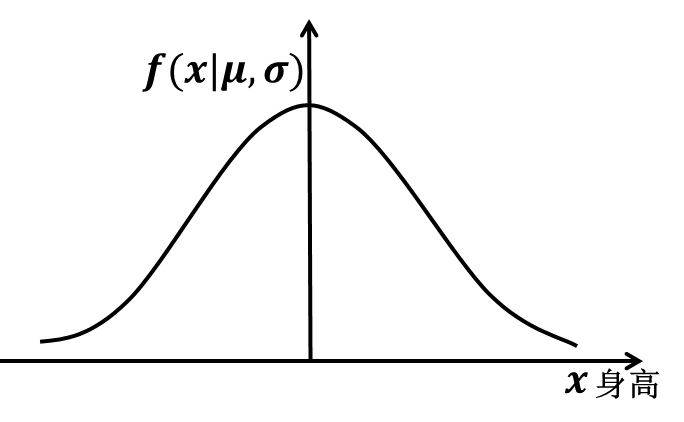
\includegraphics[height=3cm]{images/Height_distribution_fit.jpg}
    %         \caption{身高分布拟合示意图1}
    %         \label{fig:身高分布拟合示意图1}
    %         \end{figure}
    \par
    在给出$x_1,x_2,\dots,x_n$后,用$m_i$表示落在$x_i$邻域$x_i\pm h$的样本个数,$p_i = \frac{m_i}{n}$表示落在$x_i$邻域$x_i\pm h$的频率(可能/概率),令$h\rightarrow 0$,$p_i$是$x_i$处的真实值,$f(x_i|\mu,\sigma)$就是要拟合(逼近/估计)$p_i$,如图(\ref{fig:身高分布拟合示意图2})所示
            \begin{figure}[H]
            \centering
            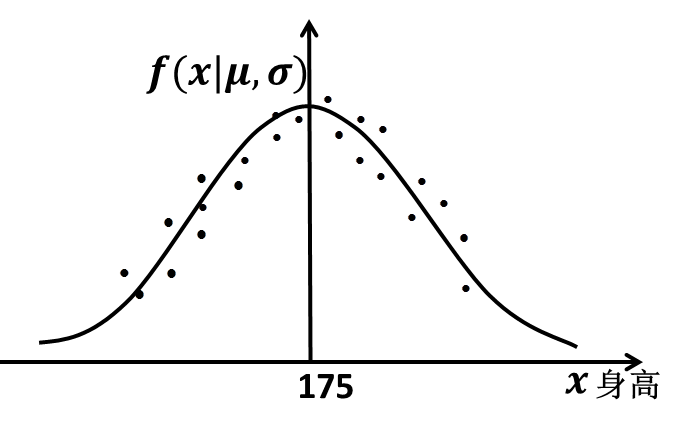
\includegraphics[height=3cm]{images/Height_distribution_fit2.jpg}
            \caption{身高分布拟合示意图}
            \label{fig:身高分布拟合示意图}
            \end{figure}
    % \textcolor[rgb]{1 0 0}{todo:图片:身高分布拟合示意图2}\\
    很自然的有OLS估计:我们使离差平方和最小,有
    \begin{align*}
    \min_{\mu,\sigma} \ J(\mu,\sigma)= \sum_{i = 1}^n \left( f(x_i) - p_i \right) ^2
    \end{align*}
    其中:在$h$给定后,样本给定后,$p_i$是一常量,而$f(x|\mu,\sigma) = \frac{1}{\sqrt{2\pi \sigma^2}} e^{- \frac{(x-\mu)^2}{2\sigma^2}  }$。
    我们可以用最简单的(不用推导的:例如GA,PSO)方法求解$\mu,\sigma^2$,易解。但是,在OLS中,我们可能不能求其显式估计量表达式。
    \par
    方法三:下面,我们来介绍第三种估计思想 - 极大似然估计。在已知总体分布$f:x\sim N(\mu,\sigma^2)$,但不知分布参数$\mu,\sigma$时,我们从安财男生中开始(有放回)抽取样本$x_1,x_2,\dots,x_n$,设第$i$个样本为$x_i$,则$x_i$被抽中的概率为$p(x_i)$。注意,这里的样本$x_i$是身高。如果给出的$\mu,\sigma^2$比较好,则每次样本出现的概率都很大,比如我们给定了$\mu,\sigma$,并且这个恰好就是真实的样本分布,那么,我们从这个样本分布中采样的话,概率大的样本更容易被挑中。极端地,可能$n$次都挑中$x_i = 1.75$(如果1.75是分布均值的话)。优良的$\mu,\sigma$可以使样本的出现概率(联合概率)最大,假设样本独立同分布,有
    \begin{align*}
    \max_{\mu,\sigma} \ J(\mu,\sigma)&\triangleq L(x_1,x_2,\dots,x_n) \\
    &= p(x_1)p(x_2)\dots p(x_n)\\
    &= \prod_{i = 1}^np(x_i)\\
    &= \prod_{i = 1}^n \frac{1}{\sqrt{2\pi\sigma^2}} e^{-\frac{(x_i-\mu)^2}{2\sigma^2}}
    \end{align*}
    \par
    在$x_1,x_2,\dots,x_n$给出后,$L$仅是$\mu,\sigma$的函数,我们在参数$\mu,\sigma$的参数空间$\Theta$中求最好的$\mu,\sigma$使得目标$L$最大$\max L$。由于有连乘$\prod$,我们将$L$取对数$\log L$,然后再关于$\mu,\sigma$求导(求极值),有
    \begin{align*}
    &\hat{\mu} = \frac{1}{n}\sum x_i\\
    &\hat{\sigma}^2 = \frac{1}{n}\sum (x_i - \hat{\mu})^2
    \end{align*}
    问:1.同一参数有不同的估计方法,那么那种方法好?即如何评价估计量的质量。2.估计量$\hat{\mu}$是样本的函数,每个一组样本$x_1,x_2,\dots,x_n$,都会有一个估计值,样本是随机的,所以估计量$\hat{\mu}$也是随机的,那么随机变量的分布(统计特性)如何?
\section{单总体参数估计与检验}
    \subsection{正态总体方差已知的单总体均值的估计与检验}
        \label{sec:单总体均值的估计与检验}
        \par
        下面,我们来具体的处理一下安财男生身高问题。我们假设身高$x$服从正态分布$N(\mu,\sigma^2)$,并且假设分布的方差$\sigma^2$已知。给出具体样本$x_1,x_2,\dots,x_n$后,有
        \begin{align*}
        \hat{\mu} = \frac{1}{n} \sum_{i = 1}^n x_i
        \end{align*}
        \par
        前面,我们提到过估计量$\hat{\mu}$是一个随机变量,下面,我们来研究一下$\hat{\mu}$的分布情况。
        \begin{align*}
        &\because x_i\sim N(\mu,\sigma^2) \quad iid\\
        &\therefore \sum_{i = 1}^nx_i \sim N(n\mu,n\sigma^2) \quad \text{正态分布可加性}
        \end{align*}
        也即
        \begin{align*}
        n\hat{\mu}\sim N(n\mu,n\sigma^2)
        \end{align*}
        于是有
        \begin{align*}
        &E(n\hat{\mu}) = n \mu\\
        \Rightarrow{}& E(\hat{\mu}) = \mu\\
        &Var(n\hat{\mu}) = n\sigma^2\\
        \Rightarrow{}&n^2 Var(\hat{\mu}) = n\sigma^2\\
        \Rightarrow{}&Var(\hat{\mu}) = \frac{\sigma^2}{n}
        \end{align*}
        即$\hat{\mu} = N(\mu,\frac{\sigma^2}{N})$,或者归一化写为
        \begin{align*}
        \frac{\hat{\mu} - \mu}{\sqrt{\sigma^2/n}}\sim N(0,1)
        \end{align*}
        \par
        统计量$\hat{\mu}$的分布如图(\ref{fig:估计量分布图})所示
            \begin{figure}[H]
            \centering
            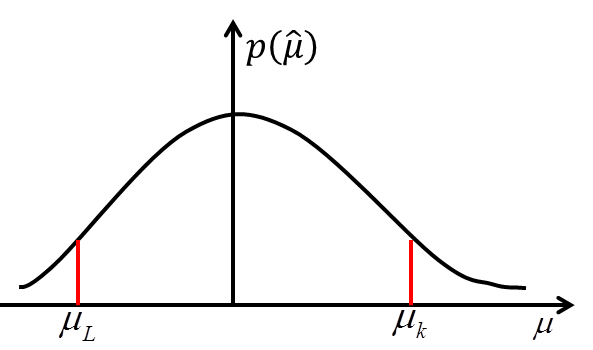
\includegraphics[height=3cm]{images/Estimation_of_the_distribution.jpg}
            \caption{估计量分布图}
            \label{fig:估计量分布图}
            \end{figure}
        % \textcolor[rgb]{1 0 0}{todo:图片:估计量分布图}
        \par
        参数$\mu$的区间估计:在上面的估计$\mu$的过程中,我们对总体均值$\mu$给出了点估计,即估计$\mu$是一个具体的值,例如:$\hat{\mu} = 1.75$。我们也可以给出$\mu$的一个估计区间,比如我们说安财男生的平均身高在$[1.70,1.80]$之间,我们可以用一个区间来估计$\mu$,我们记$\mu$的估计区间为$[\hat{\mu}_L,\hat{\mu}_K]$。从$\hat{\mu}$的分布图(\ref{fig:估计量分布图})中,我们可以看到,$\hat{\mu}$包含在估计区间$[\hat{\mu}_L,\hat{\mu}_K]$的概率为
        \begin{align*}
        P = \int_{\hat{\mu}_L}^{\hat{\mu}_K}p(\hat{\mu}) \mathrm{d}\mu
        \end{align*}
        其中:$p(\hat{\mu})$为$\mu$的密度函数。概率$P$为多次采样$\mathbf{x}$后估计区间$[\hat{\mu}_L(\mathbf{x}),\hat{\mu}_K(\mathbf{x})]$包含$\mu$的概率,其示意图如图(\ref{fig:区间估计示意图})所示
            \begin{figure}[H]
            \centering
            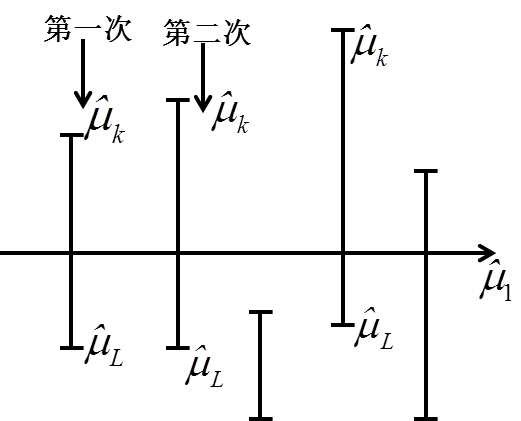
\includegraphics[height=3cm]{images/Interval_estimates.jpg}
            \caption{区间估计示意图}
            \label{fig:区间估计示意图}
            \end{figure}
        % \textcolor[rgb]{1 0 0}{todo:图片:区间估计示意图}\\
        图(\ref{fig:区间估计示意图})的横轴为总体参数$\mu$,每一个纵向线段为一次区间估计,当取$n$次区间估计时,这$n$次中会有$m = Pn$次包含$\mu$。
        \par
        参数$\mu$的假设检验:在$\sigma^2 =1$已知的情况下,我们假设安财男生身高$x$的平均值为$\mu = 0.75$。现在我们来考虑这样的假设是否合理?我们知道,在原假设成立的情况下,将样本$\mathbf{x}$带入估计量$\hat{\mu}$当中,有
        \begin{align*}
        \frac{\hat{\mu}(\mathbf{x}) - 0.75}{\sqrt{1/n}} = 0.6
        \end{align*}
        其中:$\mathbf{x}$和$n$皆已知。由$\frac{\hat{\mu} - \mu}{\sqrt{\sigma^2/n}}\sim N(0,1)$,我们可以找到$0.6$对应的概率$f(0.6)$,这里的$f$就是标准正态分布$N(0,1)$。$f(0.6)$即为样本出现的概率,即抽一次样本,样本为$\mathbf{x}$的概率,如图(\ref{fig:假设检验示意图1})所示
            \begin{figure}[H]
            \centering
            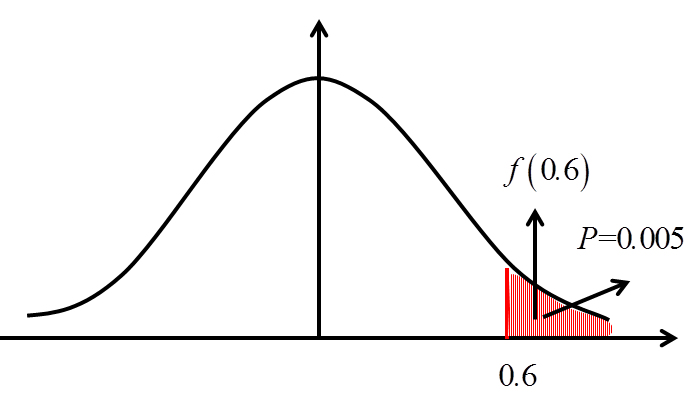
\includegraphics[height=3cm]{images/hypothetical_test1.jpg}
            \caption{假设检验示意图1}
            \label{fig:假设检验示意图1}
            \end{figure}
        % \textcolor[rgb]{1 0 0}{todo:图片:假设检验示意图}\\
        样本出现的可能性太小,即拒绝$\mu = 0.75$假设(原假设),因为$\mu$有更大的可能取其它值。为此,我们让$\mu$从$0.5$到$1.85$遍历取值,哪一个$\mu$值使样本出现的概率最大,我们就选择这个假设,这也对应了极大似然估计的思想,只有当$\hat{\mu} - \mu =0$时,样本出现的概率才最大。我们可以在检验统计量分布中设置界限(阈值)$\alpha$,如图(\ref{fig:假设检验示意图2})所示
            \begin{figure}[H]
            \centering
            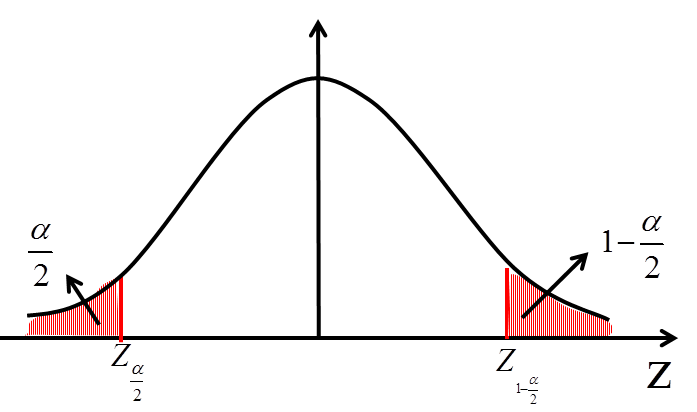
\includegraphics[height=3cm]{images/hypothetical_test2.jpg}
            \caption{假设检验示意图2}
            \label{fig:假设检验示意图2}
            \end{figure}
        当$\frac{\hat{\mu}(\mathbf{x}) - \mu}{\sqrt{1/n}} = \Delta$(其中$\mu=1.75$,$\Delta > Z_{1-\frac{\alpha}{2}}$)时,我们不能接受原假设$\mu=1.75$,称在$\alpha$显著水平下,不能接受原假设。这里的$\alpha$是一个概率,称为显著水平,$Z_{1-\frac{\alpha}{2}}$是一个样本点(横坐标$z$($z = \frac{\hat{\mu} - \mu}{\sqrt{1/n}}$)上的一个点),$P\{Z_{\frac{\alpha}{2}}<z<Z_{1-\frac{\alpha}{2}}\} = 1-\alpha$。

    \subsection{正态总体方差的估计与检验}
        \par
        我们假设$x\sim N(\mu,\sigma^2)$,$\sigma^2$未知。有样本$\mathbf{x}= \{x_1,x_2,\dots,x_n\}$,下面考虑如何依据样本来估计总体的分布参数$\sigma^2$?\\
        1、在总体参数$\mu$已知的情况下,同前,有
        \begin{align*}
        \hat{\sigma}^2 = \frac{1}{n} \sum_{i = 1}^n(x_i -\mu)^2
        \end{align*}
        2、如果$\mu$未知,我们需要用样本均值(估计量)$\hat{\mu}$来代替$\mu$,于是有
        \begin{align*}
        \hat{\sigma}^2 = \frac{1}{n-1}\sum_{i=1}^n(x_i - \hat{\mu})^2\triangleq s^2
        \end{align*}
        \par
        我们知道$s^2$是一个随机变量\footnote{本书中的$:=$、$\triangleq $、$\equiv$均表示等价},并且知道$\hat{\mu} \sim N(\mu,\sigma^2/n)$,下面,我们来求解随机变量$s^2$的分布\footnote{可以参考《数理统计引论》P4或者《数理统计学》P36定理1.3.3}。我们将样本均值$\hat{\mu}$记为$\bar{x}$,有
        \begin{align*}
        s^2 = \frac{1}{n-1}\sum_{i=1}^n(x_i - \bar{x})^2
        \end{align*}
        即
        \begin{align*}
        (n-1)s^2 &= \sum_{i=1}^n(x_i - \bar{x})^2\\
        &=\sum_{i=1}^n (x_i^2 + \bar{x}^2 -2x_i\bar{x})\\
        &=\sum_{i = 1}^n x_i^2 - (\sqrt{n}\bar{x})^2
        \end{align*}
        \par
        这里我们简单的设想一下:$\sum_{i =1 }^n x_i^2 \sim \chi^2(n)$,$(\sqrt{n}\bar{x})^2\sim \chi^2(1)$,那么,$s^2 \sim \chi^2(n-1)$。我们来详细看一下刚才的设想,$x_i \sim N(\mu,\sigma^2)$,$\bar{x}\sim N(\mu,\frac{\sigma^2}{n})$,$\sqrt{n}\bar{x}\sim N(\sqrt{n}\mu,\sigma^2)$,我们需要$x_i^2$的分布。
        \begin{lemma}[卡方分布]
        假设$x_1,x_2,\dots,x_n\overset{iid}{\sim} N(0,1)$,则
        \begin{align*}
        X = \sum_{i=1}^n x_i^2 \sim \chi^2 (n)
        \end{align*}
        其中:$n$为卡方分布$\chi^2$的自由度。
        \end{lemma}
        \par
        下面,我们来看一下卡方分布$\chi^2(n)$的分布函数和密度函数。设$k(x|n)$为密度函数,$K(x|n)$为分布函数,当$x \leqslant 0$时,有$K(x|n) = 0$;当$x>0$时,有
        \begin{align}
        \label{卡方分布公式}
        K(x|n) &= P(X<x) \notag \\
        &= P\left\{\sum_{i =1}^n x_i^2<x\right\} \notag \\
        &=P\left\{ \mathbf{x}^\mathrm{T}\mathbf{x}<x \right\}\notag \\
        &=(-2\pi)^{-\frac{n}{2}}\int\dots\int_B\exp \left( -\frac 12 \mathbf{x}^\mathrm{T}\mathbf{x} \right) \mathrm{d}\mathbf{x}
        \end{align}
        其中:$B$为$R^n$的球体$\{\mathbf{x}:\mathbf{x}^\mathrm{T}\mathbf{x}<x\}$,而$\mathrm{d}\mathbf{x} = \mathrm{d}x_1\dots\mathrm{d}x_n$。
        作为示例,我们先来看一个二维情况:
        \begin{align*}
        \iint\limits_{x_1^2+x_2^2<x} e^{-\frac 12 (x_1^2+x_2^2)}\mathrm{d}x_1\mathrm{d}x_2
        \end{align*}
        令
        \begin{align*}
        \left\{
        \begin{aligned}
        x_1= r\cos \theta\\
        x_2 = r\sin\theta
        \end{aligned}
        \right.
        \end{align*}
        于是有
        \begin{align*}
        \int_0^{2\pi}\mathrm{d}\theta\int_0^{\sqrt{x}} r e^{-\frac 12 r^2}\mathrm{d}r
        \end{align*}
        \par
        将(\ref{卡方分布公式})转化为球面坐标,不难看出$\mathbf{x}$被积函数将变为$D(\theta_1,\dots,\theta_{n-1})e^{-r^2/2}r^{n-1}$的形状,且$(\theta_1,\dots,\theta_{n-1})$的积分范围与$r$无关,于是有
        \begin{align*}
        K(x|n) = C_n \int_0^{\sqrt{x}}e^{-r^2/2}r^{n-1}\mathrm{d}r
        \end{align*}
        其中:$C_n$只与$n$有关。为求$C_n$,由分布$K(x\rightarrow \infty) =1$,令$x\rightarrow \infty$,有
        \begin{align*}
        1 &= C_n\int_0^\infty e^{-r^2/2}r^{n-1}\mathrm{d}r \\
        &= C_n2^{\frac{n}{2}-1}\Gamma \left( \frac{n}{2} \right)
        \end{align*}
        由此得到$C_n$
        \begin{align*}
        C_n = \frac{1}{2^{\frac{n}{2}-1}\Gamma \left( \frac{n}{2} \right)}
        \end{align*}
        然后带入$K(x|n)$中,有
        \begin{align*}
        K(x|n) = \frac{1}{2^{\frac{n}{2}-1}\Gamma \left( \frac{n}{2} \right)} \int_0^{\sqrt{x}}e^{-\frac 12 r^2}r^{n-1}\mathrm{d}r
        \end{align*}
        两边对$x$求导,有
        \begin{align*}
        k(x|n) = \frac{1}{2^{\frac{n}{2}-1}\Gamma \left( \frac{n}{2} \right)}e^{-\frac{x}{2}}x^{\frac{n}{2}-1}
        \end{align*}
        卡方分布$\chi^2(x|n)$中,$n$为自由度参数,当$n$取不同值时,卡方分布的图像如图(\ref{fig:卡方分布图})所示\footnote{https://en.wikipedia.org/wiki/Chi-squared\_distribution}\footnote{图中的$k$即为$n$}
           \begin{figure}[H]
           \centering
           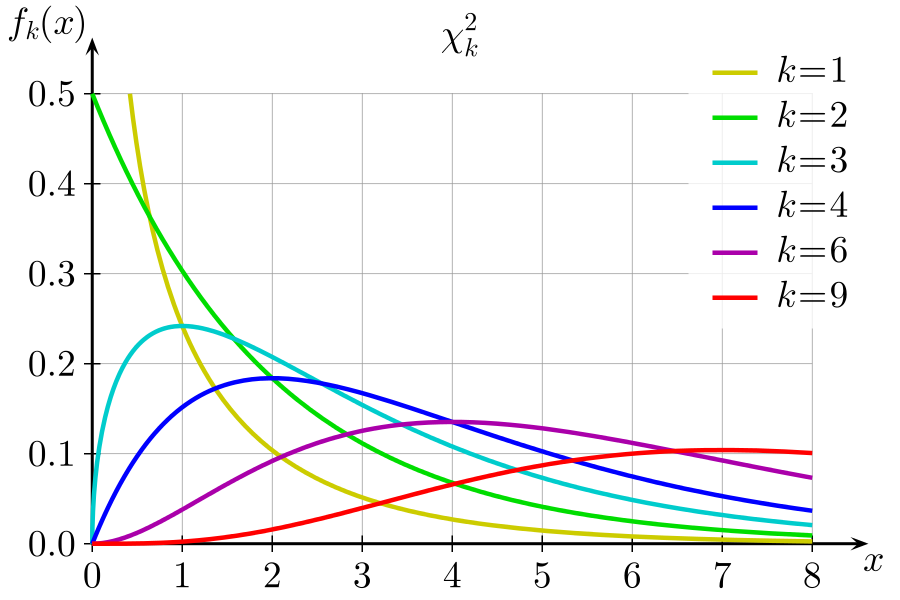
\includegraphics[width=6cm]{images/Chisquare_distribution.png}
           \caption{卡方分布}
           \label{fig:卡方分布图}
           \end{figure}
        % \textcolor[rgb]{1 0 0}{todo:matlab图片:卡方分布图}\\
        \begin{corollary}[卡方分布的一般形式1]
        在前面的卡方分布中,我们假设$x_1,x_2,\dots,x_n$独立同分布于$N(0,1)$,现在,我们来把假设放宽。假设$x_1,x_2,\dots,x_n$独立同分布于$N(0,\sigma^2)$,令$X = \sum_{i= 1}^nx_i^2$,则
        \begin{align*}
        X/\sigma^2 \sim \chi^2(n)
        \end{align*}
        \end{corollary}
        \begin{corollary}[卡方分布的一般形式2]
        假设$x_1,x_2,\dots,x_n$独立同分布于$N(\mu,\sigma^2)$,令$X = \sum_{i= 1}^nx_i^2$,则
        \begin{align*}
        X/\sigma^2 \sim \chi^2(n,r)
        \end{align*}
        其中:$r = n\frac{\mu^2}{2\sigma^2}$为非中心参数。
        \end{corollary}
        \begin{corollary}[卡方分布的一般形式3]
        假设$x_1,x_2,\dots,x_n$独立,$x_i\sim N(\mu_i,\sigma^2),i = 1,2,\dots,n$,令$X = \sum_{i= 1}^nx_i^2$,则
        \begin{align*}
        X/\sigma^2 \sim \chi^2(n,\delta)
        \end{align*}
        其中:
        \begin{align*}
        \delta = \left( \frac{\sum_{i = 1}^n \mu_i^2 }{\sigma}\right)^{1/2}
        \end{align*}
         为非中心参数。
        \end{corollary}
        \par
        下面,我们继续来求解$s^2$的分布。根据正态分布标准化,我们有
        \begin{align*}
        &x_i \sim N(\mu,\sigma^2)\\
        &\frac{x_i - \mu}{\sigma}\sim N(0,1)\\
        &\sqrt{n}\bar{x}\sim N(\sqrt{n}\mu,\sigma^2)\\
        &\frac{\sqrt{n}\bar{x} - \sqrt{n}\mu}{\sigma} \sim N(0,1)
        \end{align*}
        由卡方分布,我们有
        \begin{align*}
        \sum_{i = 1}^n \frac{(x_i - \mu)^2}{\sigma^2}\sim \chi(n)\\
        \frac{[\sqrt{n}(\bar{x}-\mu)]^2}{\sigma^2} \sim \chi(1)
        \end{align*}
        并且
        \begin{align*}
        &\sum_{i = 1}^n (x_i - \mu)^2 - [\sqrt{n}(\bar{x}-\mu)]^2\\
        =&\sum x_i^2+n\mu^2 -2\mu \sum x_i - n(\bar{x}-\mu)^2\\
        =&\sum x_i^2 - \mu^2 - (\sqrt{n}\bar{x})^2+\mu^2\\
        =&\sum x_i^2- (\sqrt{n}\bar{x})^2\\
        =&: (n-1)s^2
        \end{align*}
        于是
        \begin{align*}
        \frac{(n-1)s^2}{\sigma^2} = \sum_{i = 1}^n \frac{(x_i - \mu)^2}{\sigma^2}- \frac{[\sqrt{n}(\bar{x}-\mu)]^2}{\sigma^2}\sim \chi^2 (n) - \chi^2(1)
        \end{align*}
        \begin{lemma}[卡方分布的可加性]
        设$x_1\sim \chi^2(m)$,$x_2\sim \chi^2(n)$,则$x_1+x_2 \sim \chi^2(m+n)$。
        \end{lemma}
        \par
        由上面的卡方分布的可加性,我们有
        \begin{align*}
        \frac{(n-1)s^2}{\sigma^2} \sim \chi^2(n-1)
        \end{align*}
        \par
        至此,我们得到了$s^2$的分布。利用$\frac{(n-1)s^2}{\sigma^2} \sim \chi^2(n-1)$,我们可以对总体方差$\sigma^2$做假设检验。我们(原)假设$H0:\sigma^2 = 1$,在$H0$成立的条件下,
        \begin{align*}
        T(\mathbf{x}) = \frac{(n-1)s^2(\mathbf{x})}{\sigma^2 = 1} \sim \chi^2(n-1)
        \end{align*}
        将具体样本$x_1,x_2,\dots,x_n$带入$T$,可以得到$T$的一个具体值,例如$T_1 = 0.569$。我们在卡方分布$\chi^2(n-1)$下找$T_1= 0.569$对应的概率值,例如$P_1 =0.23$,并计算p值
        \begin{align*}
        \text{p值} = 1 - P(T < 0.569)
        \end{align*}
        如果p值较小,则说明样本出现的概率较小,不能接受原假设$H0$。我们还可以设置规则$\alpha$,当$T_1>\chi^2_{1-\alpha}$时,不能接受原假设$H0$,这里的$\chi^2_{1-\alpha}$是$\chi^2$的$1-\alpha$分位数。统计上称规则$\alpha$为显著水平,一般取值$0.1$、$0.05$和$0.01$。注意,这里的p值和规则$\alpha$都是概率。
        \subsubsection{卡方分布的性质}
            卡方分布具有如下性质:
            \par
            1).均值方差。若$X\sim \chi ^2(n)$,则$E(X) = n$,$Var(X) = 2n$。
            \par
            2).若$Y_1,Y_2,\dots,Y_m$独立,$Y_i \sim \chi ^2(n_i,\delta_i)$,则
            \begin{align*}
            Y = \sum Y_i \sim \chi^2(n,\delta)
            \end{align*}
            其中:$n = \sum n_i$,$\delta^2 = \sum \delta_i^2$。
            \par
            3).若$X_1,X_2,\dots,X_n\sim \chi ^2(n)$,则当$n\rightarrow\infty$时,有
            \begin{align*}
            \frac{X_n -n }{2n} \xrightarrow{L} N(0,1)
            \end{align*}
            且$\sqrt{2X_n}- \sqrt{2n} \xrightarrow{L}N(0,1)$。其中:$\xrightarrow{L}$表示依分布收敛。
            \par
            4).若$X_i \sim \chi^2(n,\delta_i)$,$i = 1,2$,而$\delta_1>\delta_2$,则$X_1>X_2$。

    \subsection{正态总体方差未知的单总体均值的估计与检验}
        \par
        在前面的单总体均值估计部分(\ref{sec:单总体均值的估计与检验}),我们假设总体方差$\sigma^2$已知,但是在实际问题中,我们往往只能假设安财男生身高$x\sim N(\mu,\sigma^2)$,并不知道总体方差$\sigma^2$是多少,我们只能利用样本来推断(估计)总体。总体均值$\mu$的估计仍然可以使用
        \begin{align*}
        \hat{\mu}=\frac{1}{n} \sum_{i  =1}^n x_i \sim N(\mu,\sigma^2/n)
        \end{align*}
        但是总体均值的检验则不能使用下面的检验统计量
        \begin{align*}
        \frac{\hat{\mu} - \mu}{\sqrt{\sigma^2/n}} \sim N(0,1)
        \end{align*}
        因为这里的总体方差$\sigma^2$不知道。很自然的,我们想到用样本方差$s^2$代替总体方差,那么新的检验统计量为
        \begin{align*}
        \frac{\hat{\mu} - \mu}{\sqrt{s^2/n}}
        \end{align*}
        \par
        接下来要讨论的问题是:新的统计量的分布是什么?我们来简单看一下随机变量$\frac{\hat{\mu} - \mu}{\sqrt{s^2/n}}$,分式上面的$\hat{\mu} - \mu$是正态分布,分式下面的$\sqrt{s^2/n}$是近似的卡方分布(开平方),下面,我们来详细推导这个随机变量的分布。
        \par
        设
        \begin{align*}
        T = \frac{\hat{\mu} - \mu}{\sqrt{s^2/n}}
        \end{align*}
        已知$\frac{\hat{\mu} - \mu}{\sqrt{\sigma^2/n}}\sim N(0,1)$,$\frac{(n-1)s^2}{\sigma^2} \sim \chi ^2(n-1)$,于是有
        \begin{align*}
        T &= \frac{\hat{\mu} - \mu}{\sqrt{\sigma^2/n}} \frac{\sqrt{\sigma^2/n}}{\sqrt{s^2/n}}\\
        &= \frac{\hat{\mu} - \mu}{\sqrt{\sigma^2/n}}\sqrt{\frac{\sigma^2}{s^2}}\\
        &=\frac{\frac{\hat{\mu} - \mu}{\sqrt{\sigma^2/n}}}{\sqrt{\frac{s^2}{\sigma^2}}}
        \end{align*}
        我们下面要求$\sqrt{\frac{s^2}{\sigma^2}}$。令$Z = \sqrt{\frac{s^2}{\sigma^2}}$,设其密度函数为$f_Z(z)$,分布函数为$F_Z(z)$,当$z \leqslant 0$时,$f_Z(z) = 0$,当$z>0$时,有
        \begin{align*}
        F_Z(z) &= P\{Z \leqslant z\}\\
        &=P\left\{\sqrt{\frac{s^2}{\sigma^2}} \leqslant z\right\}\\
        &=P\left\{\frac{s^2}{\sigma^2}\leqslant z^2\right\}\\
        &=P\left\{ \frac{ns^2}{\sigma^2}<n z^2 \right\}\\
        &=F_Y(nz^2)
        \end{align*}
        上式中,我们令$Y = \frac{ns^2}{\sigma^2} \sim \chi^2(n)$。于是有$Z$的密度函数为
        \begin{align*}
        f_Z(z) &= F_Z'(z)\\
        &= F_Y(nz^2)'_z\\
        &=f_Y(nz^2)(2nz)\\
        &=\frac{1}{2^{\frac{n}{2}-1} \Gamma \left( \frac{n}{2} \right) } n^{\frac{n}{2}}z^{n-1}e^{-\frac{nz^2}{2}} \quad z>0
        \end{align*}
        \par
        令$X = \frac{\hat{\mu} - \mu}{\sqrt{\sigma^2/n}}$,则$T = X/Z$。现在,我们知道了$X,Z$的分布函数,要求二者商的分布函数,引入随机变量商的分布:
        \begin{lemma}[随机变量商的分布]
        设$x_1\sim g(x)$,$x_2\sim h(x)$,且二者之间相互独立。令$z = \frac{x_1}{x_2}$,则随机变量$z$的密度函数为
        \begin{align*}
        f(x)=\int_0^\infty t g(xt)h(t)\mathrm{d}t
        \end{align*}
        \end{lemma}
        \par
        由上面的随机变量商的分布,我们有$T = X/Z$的分布
        \begin{align*}
        f_T(t) &= \int_{-\infty}^{\infty}|z|f_Z(z)f_X(zt)\mathrm{d}z\\
        &=\int_0^{\infty}z\frac{1}{\sqrt{2\pi}}e^{-\frac{z^2t^2}{2}}  \frac{1}{2^{\frac{n}{2}-1} \Gamma \left( \frac{n}{2} \right) } n^{\frac{n}{2}}z^{n-1}e^{-\frac{nz^2}{2}}\mathrm{d}z\\
        &=\frac{n^{\frac{n}{2}}}{\sqrt{2\pi}2^{\frac{n-1}{2}}\Gamma(\frac{n}{2})} \int_0^\infty z^ne^{-\frac{z^2}{2}(n+t^2)}\mathrm{d}z\\
        &\xlongequal{\text{令}u = \frac{n+t^2}{2}z^2}\frac{1}{\sqrt{n\pi}\Gamma \left( \frac{n}{2}\right)\left(1+\frac{t^2}{n} \right) ^{\frac{n+1}{2}}} \int_0^\infty u^{\frac{n+1}{2}-1}e^{-u}\mathrm{d}u\\
        &=\frac{\Gamma(\frac{n+1}{2})}{\sqrt{n\pi}\Gamma(\frac{n}{2})} \left( 1+\frac{t^2}{n} \right)^{-\frac{n+1}{2}}
        \end{align*}
        上式中用到了$\Gamma$函数的表达式
        \begin{align*}
        \Gamma(\alpha) = \int_0^\infty x^{\alpha-1}e^{-x}\mathrm{d}x
        \end{align*}
        也是因为要拼凑$\Gamma$函数,所以有变换$u = \frac{n+t^2}{2}z^2$。我们用$t(n)$来表示$t$分布的密度函数$f_T(t)$,其中,$n$为自由度参数,当$n$取不同值时,$t$分布密度函数图像如T分布密度函数图(\ref{fig:T分布密度函数图})所示\footnote{https://en.wikipedia.org/wiki/Student\%27s\_t-distribution}
           \begin{figure}[H]
           \centering
           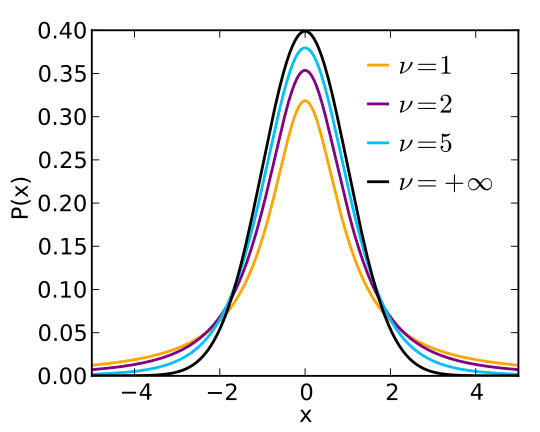
\includegraphics[width=6cm]{images/T_distribution_density_func.png}
           \caption{$\Gamma$分布密度函数图}
           \label{fig:T分布密度函数图}
           \end{figure}
        % \textcolor[rgb]{1 0 0}{todo:matlab图片:T分布密度函数图}\\
        我们利用$T = X/Z\sim t(n-1)$可以进行方差未知时总体均值$\mu$的假设检验,这里不再叙述。
        \subsubsection{t分布的性质}
            $t$分布具有以下性质:
            \par
            1).自由度为1的$t$分布为柯西分布,它的期望不存在。
            \par
            2). $n>1$时,$t$分布的数学期望存在,并且为0。
            \par
            3). $n>2$时,$t$分布的方差存在,并且为$n/(n-2)$。
            \par
            4).自由度$n$越大,$t(n)$分布越接近标准正态分布。当$n\rightarrow \infty$时,$t(n)$分布的极限分布为标准正态分布。一般认为,当$n>30$时,$t(n)$可以用标准正态分布近似。
    \subsection{两总体方差大小的估计与检验}
        \label{sub:两总体方差大小的估计与检验}
        \par
        传说中,统计有三大分布:卡方分布$\chi^2$、$t$分布和$F$分布。前面,我们给出了$\chi^2$分布和$t$分布的简单形式,下面,我们引出$F$分布。
        \par
        蚌埠有5所大学,我们选择蚌埠医学院和安财来做研究。我们想知道2所高校男生身高离散程度(方差)的差异,直接的说,两所高校男生身高的方差是否相同,谁大谁小?设安财男生身高总体为$x_1 \sim N(\mu_1,\sigma_1^2)$,蚌医男生身高总体为$x_2\sim N(\mu_2,\sigma_2^2)$,不论总体均值是否知道,在$\sigma_1^2,\sigma_2^2$未知的情况下,问$\sigma_1^2,\sigma_2^2$的关系如何?有样本$x_{11},x_{12},\dots,x_{1n};x_{21},x_{22},\dots,x_{2m}$,如果仅考虑参数估计问题,我们用样本把$\sigma_1^2,\sigma_2^2$估计出来$\hat{\sigma}_1^2,\hat{\sigma}_2^2$,然后比较大小即可。如果是假设检验问题,我们假设二者的方差相等$H0:\sigma_1^2=\sigma_2^2$,我们可以尝试构造下面两种检验统计量
        \begin{align*}
        &T_1 = \frac{\hat{\sigma_1}^2}{\hat{\sigma_2}^2}\\
        &T_2 = \hat{\sigma_1}^2 - \hat{\sigma_2}^2
        \end{align*}
        如果假设$H0$成立,那么$T_1$取值应该在$1$左右,$T_2$取值应该在$0$左右。但是,对于假设检验,我们不仅仅要看统计量的取值,更要求解统计量的分布,对于第二个统计量$T_2$,我们知道$\frac{n\hat{\sigma}_1^2}{\sigma_1^2} \sim \chi^2(n)$,$\frac{m\hat{\sigma}_2^2}{\sigma_2^2} \sim \chi^2(m)$,但是由于方差$\sigma^2$未知,我们不能求出具体的统计量值。对于第一个统计量$T_1$
        \begin{align*}
        T_1 &= \frac{\hat{\sigma_1}^2}{\hat{\sigma_2}^2}\\
        &=\frac{\frac{n\hat{\sigma}_1^2}{\sigma_1^2}\frac{\sigma_1^2}{n}}{\frac{m\hat{\sigma}_2^2}{\sigma_2^2}\frac{\sigma_2^2}{m}}
        \end{align*}
        令$X = \frac{n\hat{\sigma}_1^2}{\sigma_1^2} \sim \chi^2(n)$,$Y=\frac{m\hat{\sigma}_2^2}{\sigma_2^2} \sim \chi^2(m)$,则
        \begin{align*}
        T_1 = \frac{X}{Y}\frac{m}{n}
        \end{align*}
        \par
        可以看出,统计量$T_1$是随机变量商的形式,我们可以用随机变量商的分布来求解。有两种思路:1、将$\frac{X}{n}$和$\frac{Y}{m}$视为两个随机变量,先求各自的分布,然后再求二者商的分布,由于$X,Y$的相似性,我们只需要求解一个就可以了。2、将$\frac{X}{Y}$和$\frac{m}{n}$视为两部分,先求$\frac{X}{Y}$的商形式的分布,再求$T_2$。
        \par
        对于第一种方法:我们知道$X\sim \chi^2(n)$,$Y\sim \chi^2(m)$,令$X_1 = \frac{X}{n}$,其分布函数为$F_{X_1}(x_1)$其密度函数为$f_{X_1}(x_1)$。
        \begin{align*}
        F_{X_1}(x_1) &= P\{X_1<x_1\}\\
        &=P\left\{\frac{X}{n} <x_1\right\}\\
        &=P\{X < nx_1\}\\
        &=F_X(nx_1)\\
        &=\int_0^{nx_1}\chi^2\mathrm{d}x
        \end{align*}
        其中:$\chi^2$为卡方分布密度函数。$X_1$密度函数为
        \begin{align*}
        f_{X_1}(x_1) = F_{X_1}(x_1)'_{x_1} &= F_X(nx_1)'_{x_1}\\
        &=f_X(nx_1)n
        \end{align*}
        上式最后的求导是积分限含参变量的求导,可以继续求解,这里不再叙述。
        \par
        对于第二种方法:首先,我们导出$Z=X_1/X_2$的密度函数。记$p_1(x),p_2(x)$为$X\sim \chi^2(n),Y\sim \chi^2(m)$的密度函数,根据独立随机变量上的分布的引理,我们有
        \begin{align*}
        f_Z(z) &= \int_0^\infty x_2 p_1(zx_2)p_2(x_2)\mathrm{d}x_2\\
        &=\frac{z^{\frac{n}{2}-1}}{\Gamma \left( \frac{n}{2} \right) \Gamma \left( \frac{m}{2} \right)2^{\frac{n+m}{2}}}\int_0^\infty x_2^{\frac{n+m}{2}-1}e^{-\frac{x_2}{2}(1-z)}\mathrm{d}x_2\\
        &\xlongequal{\text{令}u = \frac{x_2}{2}(1+z)}\frac{z^{\frac{n}{2}-1}(1+z)^{-\frac{n+m}{2}}}{\Gamma \left( \frac{n}{2} \right) \Gamma \left( \frac{m}{2} \right)}\int_0^\infty  u^{\frac{m+n}{2}-1}e^{-u}\mathrm{d}u\\
        &=\frac{\Gamma \left( \frac{n+m}{2} \right) }{\Gamma \left( \frac{n}{2} \right) \Gamma \left( \frac{m}{2} \right)} z^{\frac{n}{2}-1}(1+z)^{-\frac{n+m}{2}} \quad z>0
        \end{align*}
        然后,我们导出$T_1 = Z\frac{m}{n}$的密度函数。对于$y>0$,有分布函数
        \begin{align*}
        F_{T_1}(y) &= P\{T_1<y\}\\
        &=P\left\{Z\frac{m}{n}<y\right\}\\
        &=P\left\{Z<\frac{n}{m}y\right\}\\
        &=F_Z\left(\frac{n}{m}y\right)
        \end{align*}
        分布函数对$y$求导,有
        \begin{align*}
        f_{T_1}(y) &= F_{T_1}(y)'_y\\
        &= F_Z\left(\frac{n}{m}y\right)'_y\\
        &=f_Z\left(\frac{n}{m}y\right)\frac{n}{m}\\
        &=\frac{\Gamma \left( \frac{n+m}{2} \right) }{\Gamma \left( \frac{n}{2} \right) \Gamma \left( \frac{m}{2} \right)} \left(\frac{n}{m}y\right)^{\frac{n}{2}-1}\left(1+\frac{n}{m}y\right)^{-\frac{n+m}{2}} \frac{n}{m}\\
        &=\frac{\Gamma \left( \frac{n+m}{2} \right) }{\Gamma \left( \frac{n}{2} \right) \Gamma \left( \frac{m}{2} \right)}\left(\frac{n}{m}\right)^{\frac{n}{2}}y^{\frac{n}{2}-1}\left(1+\frac{n}{m}y\right)^{-\frac{n+m}{2}}
        \end{align*}
        我们记$F$分布为$F(n,m)$,其中,$n,m$是分布的自由度。

        \subsubsection{F分布的性质}
            $F$分布具有如下性质:
            \par
            1). $m>2$时,$F$分布的数学期望存在,且为$m/(m-2)$。
            \par
            2). $m>4$时,$F$分布的方差存在,且为$\frac{2m^2(n+m-2)}{n(n-2)^2(m-4)}$。
            \par
            3).若$F\sim F(n,m)$,则$\frac{1}{F}\sim F(m,n)$。
            \par
            4).若$t\sim t(n)$,则$t^2\sim F(1,n)$。

\section{方差分析}
    \subsection{单因素方差分析}
        \par
        方差分析用于研究分类变量对连续变量的影响。前面,在研究安财男生身高时,我们是从学校男生中进行随机抽样的。现在,我们对随机抽取的样本进行标记,标记每个男生所在的学院,假设共有4个学院,则对每个样本(男生)而言,除了有“身高”连续变量外,还有“学院”分类变量,其数据结构如图(\ref{fig:安财4个学院男生身高数据表})所示。当然,我们也可以直接从4个学院中各取相同数量的男生。
            \begin{figure}[H]
            \centering
            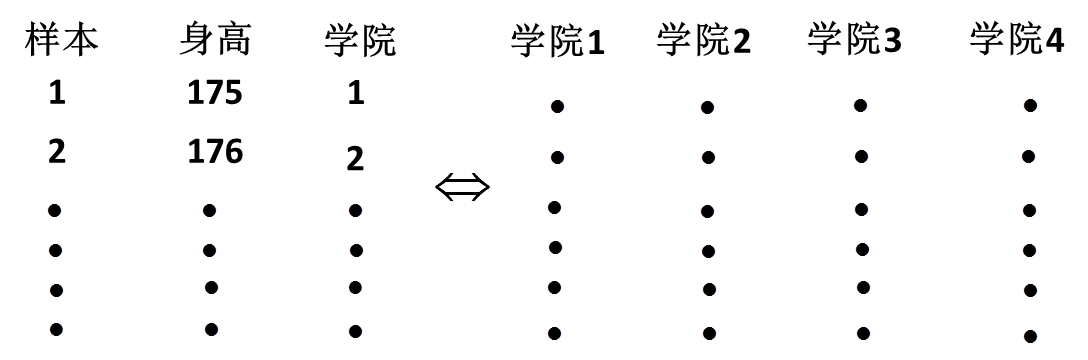
\includegraphics[height=3cm]{images/boys_height_data_sheet.jpg}
            \caption{安财4个学院男生身高数据表}
            \label{fig:安财4个学院男生身高数据表}
            \end{figure}
        % \textcolor[rgb]{1 0 0}{todo:图片:安财4个学院男生身高数据表}
        \par
        现在要研究不同学院男生身高是否有差异?也即学院变量是否影响身高变量。设分类变量(学院)为$A$(factor A),$k$为学院种类数,有$A_1,A_2,A_3,A_4$;设身高变量为$x$,学院$A_i$的样本为$x_i$,样本数为$n_i$,学院$A_i$的第$j$个样本可以表示为$x_{ij}$,我们假设$x_i\sim N(\mu_i,\sigma_i^2)$,并假设$\sigma_1 = \sigma_2 = \sigma_3 = \sigma_4$。现在,我们可以进行假设检验,我们(原)假设:不同学院男生身高均值相同,或者说所有$x_{ij}$均来自同一正态总体,即$H0:\mu_1=  \mu_2=\mu_3=\mu_4$。逆假设为:$H1:\exists i,j\in k,\mu_i \neq \mu_j$。
        \par
        下面,我们要构造检验统计量。如果$H0$成立(为真),各学院男生身高均值相等,那么样本均值也应该接近$\bar{x}_1 \approx \bar{x}_2\approx\bar{x}_3 \approx \bar{x}_4 \approx \bar{\bar{x}}$,这里的$\bar{\bar{x}}$是所有男生身高的均值。依据各组身高方差相等的假设,并且在各组样本量差别不大的情况下,我们有
        \begin{align*}
        \sum(x_{1j} - \bar{x}_1)^2 \approx \sum(x_{2j} - \bar{x}_2)^2  \approx \sum(x_{3j} - \bar{x}_3)^2  \approx \sum(x_{4j} - \bar{x}_4)^2
        \end{align*}
        我们称
        \begin{align*}
        SSE = \sum_{i=1}^k \sum_{j=1}^{n_i} (x_{ij}-\bar{x}_i)^2
        \end{align*}
        为组内离差平方和,SSE为sum of squres of error的缩写。
        称
        \begin{align*}
        SST = \sum_i\sum_j(x_{ij} - \bar{\bar{x}})
        \end{align*}
        为总的离差平方和,这里的SST是 sum of squres of total的缩写。二者相减,有
        \begin{align*}
        SST - SSE &= SSA\\
        &=\sum_{i=1}^kn_i(\bar{x}_i - \bar{\bar{x}})^2
        \end{align*}
        称$SSA$为组间离差平方和,SSA是 sum of squres of factor A的缩写。可以看出,在原假设$H0$成立的情况下,有$SST = SSE$,即$SSA = 0$。只要$SSA$不等于$0$,我们就说分类变量$A$影响身高$x$,不过,我们要讨论这种影响是否显著。根据前面介绍的卡方分布,我们有
        \begin{align*}
        \frac{(n-1)SST}{\sigma^2} \sim \chi^2(n-1)\\
        \frac{(k-1)SSA}{\sigma^2} \sim \chi^2(k-1)\\
        \frac{(n-k)SSA}{\sigma^2} \sim \chi^2(n-k)
        \end{align*}
        但是由于$\sigma^2$未知,无法计算出具体的检验统计量值,所以我们构造$F$分布
        \begin{align*}
        &F_1 = \frac{SSE}{SST}\\
        &F_2 = \frac{SSA/(k-1)}{SSE/(n-k)} \sim F(k-1,n-k)
        \end{align*}
        \par
        可以尝试证明统计量$F_2$的分布$F(k-1,n-k)$。下面,我们给出分类变量$A$对$x$的影响强度的度量
        \begin{align*}
        R^2 = \frac{SSA}{SST}\in [0,1]
        \end{align*}
        当$R^2 = 1$时,表明$A$强烈影响$x$;当$R^2 = 0$,表明$A$不影响$x$。
    \subsection{方差分析的多重比较}
        \par
        在前面的单因素方差分析当中,我们检验了各个学院男生身高均值是否相等,其原假设为$H0:\mu_1=\mu_2=\mu_3=\mu_4$。如果检验的结果没有接受原假设,那么,接下来我们就要考虑:是哪一个学院男生身高平均值特别,还是所有学院的身高均值都不相同?对于这个问题,我们有如下思路:
        \par
        我们仍然从假设检验做起,现在的目标是找到与众不同的$\mu_i$。共有4个学院,我们可以两个学院两个学院的进行检验,检验$12,13,14,23,24,34$六组的两两总体的均值是否相同。对于第$i$组和第$j$组\\
        \textbf{Step1}:原假设$H0: \mu_i = \mu_j$,备择假设$H1:\mu_i \neq \mu_j$。\\
        \textbf{Step2}:构建统计量。我们知道
        \begin{align*}
        &\hat{\mu}_i \sim N(\mu_i,\sigma^2/n_i)\\
        &\hat{\mu}_j \sim N(\mu_j,\sigma^2/n_j)\\
        &\hat{\mu}_i - \hat{\mu}_j \sim N\left(\mu_i-\mu_j,\frac{(n_i+n_j)\sigma^2}{n_in_j}\right)
        \end{align*}
        我们令
        \begin{align*}
        T = \frac{(\hat{\mu}_i - \hat{\mu}_j) - (\mu_i-\mu_j)}{\sqrt{\frac{(n_i+n_j)\sigma^2}{n_in_j}}} \sim N(0,1)
        \end{align*}
        在各组方差相等但未知的情况下(注意:这是前面单因素方差分析的假设),上式的$\sigma^2$未知,用样本方差代替,有$T \sim t(n_i+n_j-1)$。\\
        \textbf{Step3}:在$H0$为真时,将得到的样本带入$T$中,即可进行检验。
        \par
        在所有两两分组检验结束后,会得到一个表格(\ref{tab:方差分析多重比较结果表})
        \begin{table}[H]\caption{方差分析多重比较结果表}
        \label{tab:方差分析多重比较结果表}
        \centering
        \begin{tabular}{c|cccc}% 需要引入 tabularx 宏包;表格总宽度一定要设置
        组均值 & ${\mu}_1$ & ${\mu}_2$ & ${\mu}_3$ & ${\mu}_4$ \\
        \hline
        ${\mu}_1$ & 1 & 1 & 1 & 0\\
        ${\mu}_2$ & {} & 1 & 0 & 0\\
        ${\mu}_3$ & {} & {} & 1 & 0\\
        ${\mu}_4$ & {} & {} & {} & 1\\
        \end{tabular}
        \end{table}
        % \textcolor[rgb]{1 0 0}{todo:图片:方差分析多重比较结果表}\\
        表(\ref{tab:方差分析多重比较结果表})中的$1$表示不能拒绝原假设$H0$,$0$表示拒绝原假设。从表中可得到的结论为$(1,4),(2,3),(2,4),(3,4)$组的均值有显著差异。存疑:1与2同,1与3同,2与3不同?
        \par
        常用的多重比较有两种方法:一个是费希尔提出的最小显著差异方法(LSD),一个是N-K检验。LSD的基本步骤和上面的步骤相似,不过其检验统计量为
        \begin{align*}
        T = \frac{\hat{\mu}_i - \hat{\mu}_j}{\sqrt{MSE \left( \frac{1}{n_i}+ \frac{1}{n_j} \right) }} \sim t(n-k)
        \end{align*}
        其中:$MSE = \frac{SSE}{n-k} = \sum_i\sum_j(x_{ij} - \bar{x}_i)^2$。N-K检验是非参数统计中的方法,留在后面介绍。

    \subsection{方差齐性检验}
        \par
        常用的方差齐性检验有Bartlett检验(1937)和Levene检验(1960)。在前面(\ref{sub:两总体方差大小的估计与检验})的安财和蚌医男生身高方差比较当中,我们曾讨论过方差是否相等这个问题,并由此导出了$F$分布。但是,这仅是两个方差的比较,如果在多个总体的情况下,检验统计量就变得无能为力了。在单因素方差分析中,我们曾假设各个分组的方差相等$\sigma_1^2=\sigma_2^2=\sigma_3^2=\sigma_4^2=\sigma^2$,那如何检验各组的方差是否相等呢?下面,我们来介绍用于方差是否相等的检验-Bartlett检验,也就是SPSS中的ANOVA分析的方差齐性检验的首选检验方法。
        \par
        仍然考虑安财4个学院的男生身高数据,见图(\ref{fig:安财4个学院男生身高数据表}),定义两个量$MSE$和$GMSE$。
        \begin{align*}
        MSE &= \frac{SSE}{n-k}\\
        &= \frac{\sum_{i = 1}^k\sum_{j=1}^{n_i}(x_{ij} - \bar{x}_i)^2}{n-k}\\
        &=\frac{\sum_{i=1}^k Q_i}{n-k}\\
        &=\frac{\sum_{i=1}^ks_i^2(n_i-1)}{n-k}\\
        &=\sum_{i = 1}^k \frac{n_i-1}{n-k}s_i^2
        \end{align*}
        其中:$ Q_i$是第$i$组的离差平方和,$s_i^2$是第$i$组的样本方差,有$s_i^2 = \frac{Q_i}{n_i-1}$。从$MSE$的计算公式可以看出,$MSE$是各总体方差$s_i^2$的加权算术平均。定义$GMSE$为
        \begin{align*}
        GMSE = \sqrt[n-k]{\prod_{i = 1}^k(s_i^2)^{(n_i-1)}}
        \end{align*}
        从$GMSE$的计算公式来看,$GMSE$是各总体方差$s_i^2$的几何平均。对于算术平均数和几何平均数,我们有
        \begin{align*}
        \frac{x_1+x_2+\dots+x_n}{n} \geqslant \sqrt[n]{x_1x_2\dots x_n}
        \end{align*}
        即算术平均数大于几何平均数,只有在$x_1 = x_2 = x_n$时,等号才成立。根据算术平均数和几何平均数的这个性质,我们有
        \begin{align*}
        GMSE \leqslant MSE
        \end{align*}
        只有当各总体方差$s_i^2$相等时,等号才成立,各组方差差异越大,$GMSE$越小于$MSE$。此外,我们还可以尝试用熵来度量方差的离散程度。我们可以构建检验统计量
        \begin{align*}
        T = \frac{MSE}{GMSE}
        \end{align*}
        将$T$和$1$比较大小。同样可以构建
        \begin{align*}
        T = \ln \frac{MSE}{GMSE}
        \end{align*}
        将$T$和$0$比较大小。
        \par
        Bartlett检验的原假设为$H0:\sigma_1^2=\sigma_2^2=\sigma_3^2=\sigma_4^2=\sigma^2$,备择假设为$H1:\exists i,j\in K,\sigma_i^2 \neq \sigma_j^2$。检验统计量为
        \begin{align*}
        T \triangleq B = \frac{n-k}{C} \left( \ln MSE- \ln GMSE \right) \overset{\cdot}{\sim} \chi^2(k-1)
        \end{align*}
        其中:$C = 1+\frac{1}{3(k+1)} \left( \sum\limits_{i=1}^k\frac{1}{n_i-1} -\frac{1}{n-k} \right) $为校正数。
        \par
        修正Bartlett检验:针对样本量小于5不能用Bartlett检验的缺点,Box修正了Bartlett检验,修正后的检验统计量为
c        \begin{align*}
        B' = \frac{f_1 B C}{f_1 (A-B-C)} \overset{\cdot}{\sim} F(f_1,f_2)
        \end{align*}
        其中:$f_1 = k-1$,$f_2 = \frac{k+1}{(C+1)^2}$,$A = \frac{f_1}{2-C+2/f_2}$,$B,C$同前面介绍。
        Levene 检验是对模型残差进行组间齐性检验(残差方差齐性检验)。


    \subsection{MATLAB应用实例}
        1).单因素一元方差分析的matlab命令为
        \par
        [p,table,stats] =anova1(x,group,displayopt)\\
        其中:p为p值;table为元胞数组数据类型的方差分析表,包含组内方差、组间方差和总方差等以及他们对应的自由度、均方等等;stats为结构体,可作为后续的多重比较的输入参数;x可以为一列数据或者多列分组数据(矩阵),和前面介绍的一致;group为分组,当x为一列数据时,group的长度和x相等,用来指定x中各元素所在的组,当x为矩阵时,可以忽略group这个参数,或者用它来指定组名。displayopt设置为'off'时,不显示方差分析表table和箱线图。
        \par
        单因素方差分析的多重比较命令为
        \par
        [c,m,h,gnames] = multcompare(stats,param,$\dots$)\\
        其中:c两两比较结果矩阵,是一个多行5列的矩阵,每一行对应某两两比较结果,例如某一行为:$2,5,1.9442,8.2206,14.4971$,表示第2组和第5组进行比较,两组的均值差为8.2206,均值差的$95\%$置信区间为$[1.9442,14.4971]$,这个区间不包含0,说明在0.05显著水平下,两组之间的均值是显著差异的;m为多行两列矩阵,第1列为每组均值,第2列为相应的标准误差;h为交互式多重比较图形句柄;games是一个元胞数组,每一行对应一个组名;stats为anova返回的结构体;param为参数,其可选参数和参数值如表(\ref{tab:多重比较参数表})所示。
        \begin{table}[H]
        \caption{多重比较参数表}
        \label{tab:多重比较参数表}
        \newcolumntype{Y}{>{\centering\arraybackslash}X}% 定义自适应列的居中格式 Y, 用 X 为左对齐(自适应列)
        \begin{tabularx}{\textwidth}{|c|X|X|}% 需要引入 tabularx 宏包;表格总宽度一定要设置
        % \begin{tabular}{|>{}c<{}|>{\centering\arraybackslash}m{11em}|>{\setlength\parindent{2em}}m{28em}|}
        \toprule
         参数名& 参数值& 说明\\\midrule
        'alpha' & (0,1)内的标量 & 用来指出输出矩阵c中的置信区间和交互式图形上的置信区间的置信水平:100(1-alpha)\%.'alpha'的默认值是0.05\\\hline
        'display'  & 'on', 'off' & 用来指定是否显示交互式图形,若为'on'(默认情况),则显示图形;若为'off',则不显示图形\\\hline
        'ctype' & 'hsd'或'tukey-kramer', 'lsd'或'bonferroni', 'dunn-sidak', 'scheffe'& 用来指定多重比较中临界值的类型,实际上就是指定多重比较的方法。可用的方法有Tukey-Kramer法(默认情形)、最小显著差数法(LSD法)、Bonferroni t 检验法、Dunn-Sidak检验法和Scheffe法\\\hline
        'dimension' &正整数向量 & 对于多因素方差分析的比较检验,用来指定要比较的因素(分组变量)的序号,默认值为1,表示第1个分组变量。仅适用于stats是anovan函数的输出的情形\\\hline
        'estimate' & 依赖于生成结构体变量stats所用的函数 & 指定要比较的估计,其可能取值依赖于生成结构体变量stats所用的函数。对于anoval、anovan(多因素方差分析)、friedman(Friedman秩方差分析)和kruskalwallis(Kruskal-Wallis单因素方差分析)函数,该参数将被忽略;对于anova2(双因素方差分析)函数,'estimate'参数的可能取值为'column'(默认)或'row',表示对列均值或行均值进行比较;对于aoctool(交互式协方差分析)函数,'estimate'参数的可能取值为'slope'、'intercept'或'pmm',分别表示对斜率、截距或总体边缘均值进行比较。后面会陆续介绍这些函数的用法\\
        \bottomrule
        \end{tabularx}
        \end{table}
        % \textcolor[rgb]{1 0 0}{todo:图片:多重比较参数表}
        \par
        2).双因素一元方差分析的matlab命令为
        \par
        [p,table,stats] = anova2(x,reps,displayopt)\\
        其中:x的每一列对应因素A的一个水平(因子),每一行对应因素B的一个水平,anova2检验矩阵x的各列是否具有相同的均值,即因素A对x的影响是否显著,同时还检验x的各行是否具有相同均值;reps默认为1,当reps的取值大于1时,anova2还检验因素A和B的交互作用是否显著;p为检验的p值,如果仅考虑因素A和B,则p是一个2个元素的行向量,如果考虑A和B的交互作用,p是一个3个元素的行向量。
        \par
        在多重比较中,将参数'estimate'的值设置为'column'以对因素A进行多重比较,设置为'row'以对因素B进行多重比较。
        \par
        3).多因素一元方差分析的matlab命令为
        \par
        [p,table,stats,terms] = anovan(y,group,param,$\dots$)\\
        其中:group是一个元胞数组,每一个元胞对应一个因素,元胞长度和y相同,其元素可以是分类数据、数值和字符串等等;anovan支持的参数param和参数值paramvalue如表(\ref{tab:anovan参数表})所示,多因素一元方差分析模型的类型如表(\ref{tab:多因素一元方差分析模型表})所示
        \begin{table}[H]
        \caption{anovan参数表}
        \label{tab:anovan参数表}
        \newcolumntype{Y}{>{\centering\arraybackslash}X}% 定义自适应列的居中格式 Y, 用 X 为左对齐(自适应列)
        \begin{tabularx}{\textwidth}{|c|X|X|}% 需要引入 tabularx 宏包;表格总宽度一定要设置
        \toprule
         参数名& 参数值& 说明\\\midrule
        {'alpha'} & {(0,1)内的标量} & 用来指定置信区间的置信水平:100(1-alpha)\%。'alpha'的默认值是0.05\\\hline
        {'continuous' } & {下标变量} & 用来指明哪些分组变量被作为连续变量,而不是离散的分类变量\\\hline
        {'display'}  & {'on', 'off'} & 用来指定是否显示交互式图形,若为'on'(默认情况),则显示图形;若为'off',则不显示\\\hline
        'model' &所有可能取值如表(\ref{tab:多因素一元方差分析模型表})所列 & 用来指定所用模型的类型\\\hline
        {'nested'} & {由0和1构成的矩阵M} & 指定分组变量之间的嵌套关系。若第i个变量嵌套于第j个变量,则M(i,j)=1\\
        \bottomrule
        \end{tabularx}
        \end{table}
        \begin{table}[H]
        \caption{多因素一元方差分析模型表}
        \label{tab:多因素一元方差分析模型表}
        \newcolumntype{Y}{>{\centering\arraybackslash}X}% 定义自适应列的居中格式 Y, 用 X 为左对齐(自适应列)
        \begin{tabularx}{\textwidth}{|c|X|}% 需要引入 tabularx 宏包;表格总宽度一定要设置
        \toprule
         'model'参数取值& 模型说明\\\midrule
         & 只对N个主效应进行检验,不考虑交互效应,这是默认情况。例如考虑三因素(A,B,C)的试验,此模型对主效应A,B,C进行检验\\\hline
        {'interaction'}  & 对N个主效应和$C_N^2$个两因素进行检验。例如考虑三因素(A,B,C)的试验,此模型对主效应A,B,C和两因素交互效应AB,AC,BC进行检验\\\hline
        {'full'}  & 对N个主效应和全部交互效应进行检验。例如考虑三因素(A,B,C)的试验,此模型对主效应(A,B,C)、两因素交互效应(AB,AC,BC)和三因素交互效应ABC进行检验\\\hline
        {正整数k($k\le N$)} &当k=1时,此模型相当于'linear'模型;当k=2时,此模型相当于'interaction'模型;当2<k<N时,对N个主效应和2至k因素交互效应进行检验;当k=N时,此模型相当于'full'模型;\\\hline
        {由0和1构成的矩阵} & 用矩阵精确控制模型中的效应项。例如考虑三因素(A,B,C)的试验,有以下对应关系:[100]主效应A;[010]主效应B;[001]主效应C;[110]交互效应AB;[101]交互效应AC;[011]交互效应BC;[111]交互效应ABC。若矩阵为[010;001;011],则表示模型中有主效应项B,C以及交互效应项BC\\
        \bottomrule
        \end{tabularx}
        \end{table}
        % \textcolor[rgb]{1 0 0}{todo:图片:anovan参数表}\\
        % \textcolor[rgb]{1 0 0}{todo:图片:多因素一元方差分析模型表}\\
        在多重比较中,将参数'dimension'设置为向量,用来指定要比较的分组变量序号。
        \par
        4).单因素多元方差分析的matlab命令为
        \par
        [d,p,stats] = manova1(x,group,alpha)\\
        其中:d取值0时,接受原假设;取值为1时,拒绝原假设但无法拒绝共线性假设;取值为2时,拒绝原假设,拒绝共线假设,但无法拒绝共面假设。p为p值向量,它的第$i$个元素对应的原假设为:各组均值向量位于一个$i-1$维空间。stats结构体包含的字段如表(\ref{tab:manova1结构体字段表})所示
    \begin{table}[H]
    \caption{manova1结构体字段表}
    \label{tab:manova1结构体字段表}
    \centering
    \newcolumntype{Y}{>{\centering\arraybackslash}X}% 定义自适应列的居中格式 Y, 用 X 为左对齐(自适应列)
    \begin{tabularx}{\textwidth}{|l|X|}% 需要引入 tabularx 宏包;表格总宽度一定要设置
    \toprule
    字段名& 说明\\
    \midrule
    W  & 组内平方和及交叉乘积和矩阵 \\\hline
    B  & 组间平方和及交叉乘积和矩阵\\\hline
    T  &总平方和及交叉乘积和矩阵\\\hline
    dfW &W的自由度\\\hline
    dfB &B的自由度\\\hline
    dfT &T的自由度\\\hline
    lambda & Wilk's $\Lambda$检验统计量的观测值向量,第i个元素对应的原假设是:各组的均值向量位于一个i-1维空间\\\hline
    chisq &由Wilk's $\Lambda$检验统计量转换得到的近似卡方检验统计量的观测值向量\\\hline
    chisqdf &卡方检验统计量的自由度\\\hline
    eigenval  &使$W^{-1}B$的特征值\\\hline
    eigenvec  &使$W^{-1}B$的特征向量,它们是典型变量C的系数向量,经过了单位化,使得典型变量的组内方差为1\\\hline
    canon &典型变量C,等于XC*eigenvec ,其中XC是将X按列中心化(每列元素减去每列的均值)后得到的矩阵\\\hline
    mdist & 每个点到它的组均值的马氏距离(Mahalanobis距离)向量\\\hline
    gmdist & 各组组均值的之间马氏距离矩阵\\
        \bottomrule
    \end{tabularx}
    \end{table}
        % \textcolor[rgb]{1 0 0}{todo:图片:manova1结构体字段表}
\section{分布检验}
    \par
    在前面的单总体参数估计和检验,或者方差分析中,我们都假设总体是正态的,那么,如何检验假设是否为正态呢?或者更广泛的说,如何依据样本估计和检验总体的分布呢?下面,我们来解决分布检验问题。我们先从正态分布检验入手,再讨论指数分布,最后扩展到任意分布的检验。
    \par
    常用的分布检验方法有:1.卡方拟合优度检验(1900);2. Jarque-Bera检验(J-B正态检验);\\3. Kolmogonov-Smirnov检验;4. lillietest检验(1967);5. Shaoiro-Wilk检验,要求样本数$8 \leqslant n \leqslant 50$(1965,正态);6.Epps—Pully检验,要求$n \geqslant 8$(正态)。对于指数分布的检验,有卡方拟合优度检验和格列坚科检验等检验方法。
    \subsection{正态分布检验方法}
        \par
        一提到正态性检验,我们会第一时间想到JBtest,是的,JBtest是可行的,但这里我们先不去了解有哪些检验方法,我们来试着自己考虑一下。我们假设$x$服从正态分布,设置原假设为$H0:f(x)=N(\mu,\sigma^2)$。但是正态分布的参数$\mu,\sigma$未知,这使得我们根本无从下手,因为$H0$中,我们需要一个具体的正态分布。我们用样本均值和方差来代替$\mu,\sigma$,把假设变为$H0:f(x)=N(\hat{\mu},\hat{\sigma}^2)$。如果$x$不服从$N(\hat{\mu},\hat{\sigma}^2)$,那么$x$更不可能服从其它均值方差的正态分布。有了$\hat{\mu},\hat{\sigma}^2$,也就有了$N(\hat{\mu},\hat{\sigma}^2)$,我们将样本$\mathbf{x}$经验密度$f_n(x)$带入(关于经验密度,可以使用直方图或者其它),可能得到像图(\ref{fig:正态分布检验图})那样的情况
        \begin{figure}[H]
            \centering
            \begin{subfigure}[b]{0.3\textwidth}
                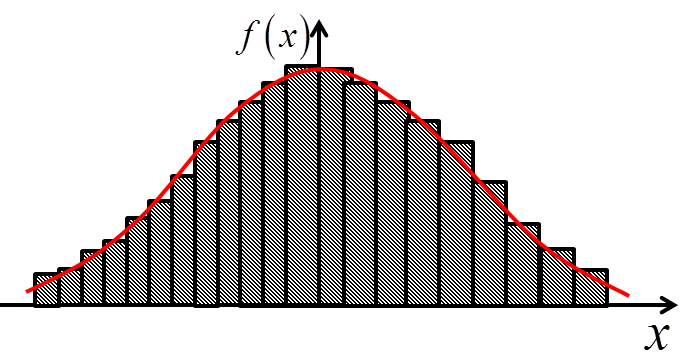
\includegraphics[width=\textwidth]{images/Normal_distribution_test1.jpg}
                \caption{}
                \label{fig:正态分布检验图1}
            \end{subfigure}
            \begin{subfigure}[b]{0.3\textwidth}
                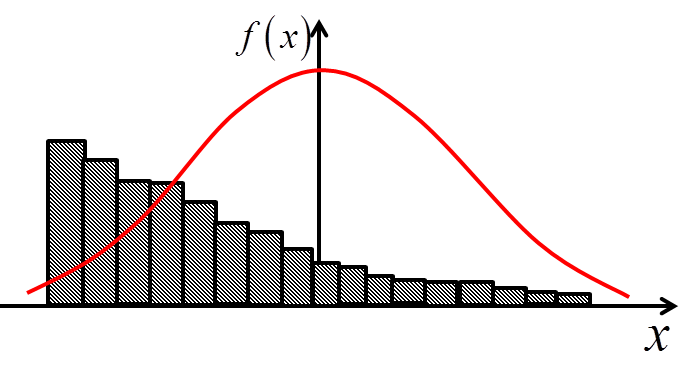
\includegraphics[width=\textwidth]{images/Normal_distribution_test2.jpg}
                \caption{}
                \label{fig:正态分布检验图2}
            \end{subfigure}
            \begin{subfigure}[b]{0.3\textwidth}
                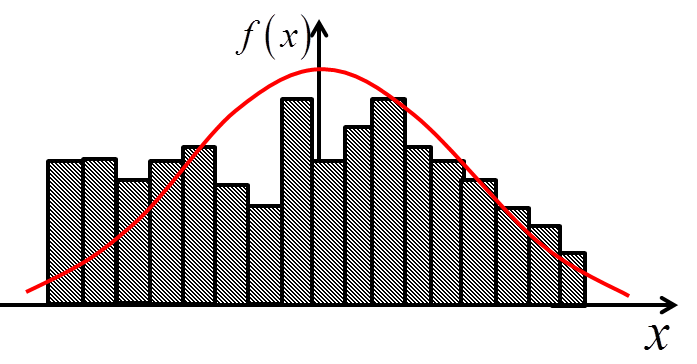
\includegraphics[width=\textwidth]{images/Normal_distribution_test3.jpg}
                \caption{}
                \label{fig:正态分布检验图3}
            \end{subfigure}
            \caption{正态分布检验图}\label{fig:正态分布检验图}
        \end{figure}
        % \textcolor[rgb]{1 0 0}{todo:图片:正态分布检验图}\\
        如果假设$H0$成立,则会有图\ref{fig:正态分布检验图}(a)的情况,如果$H0$不成立,则可能会有图\ref{fig:正态分布检验图}(b)(c)的情况。我们知道直方图$F_n(x)$和分割窗宽$h$有关,在$h$给定后,我们可以构建如下统计量
        \begin{align*}
        T = \sum_{i = 1}^n \left( f(x_i) - f_n(x_i) \right) ^2 \overset{\cdot}{\sim} \chi^2(n-1)
        \end{align*}
        离差平方和服从$\chi^2$分布是合适的。对于超参数(外来参数)$h$,我们如何确定$h$呢?我们可以让$h$逐步逼近0,然后在每个$h$下做检验,记录每次的检验效果,选取最好的。
        \par
        下面,我们介绍标准的正态分布检验方法:JBtest、Shapiro-Wilk检验和Epps-Pully检验。这里,我们不对统计量的分布进行证明。
        \par
        \textbf{JBtest}是基于这样的想法:如果$H0:f = N(\mu,\sigma^2)$成立,正态总体的偏度为0,峰度为3,那么样本的偏度应该接近0,峰度应该接近3。为此,构造检验统计量为
        \begin{align*}
        T \triangleq JB = \frac{n}{6}\left[ s^2+\frac{(k-3)^2}{4}  \right] \overset{\cdot}{\sim} \chi^2(2)
        \end{align*}
        其中:$s$为样本偏度(skewness),$k$为样本峰度(kurtosis)。对于$JB\overset{\cdot}{\sim} \chi^2(2)$,其实是这样的
        \begin{align*}
        JB = \frac{n}{6}\left[ (s-0)^2+\frac{(k-3)^2}{4}  \right] \overset{\cdot}{\sim} \chi^2(2)
        \end{align*}
        这样写的话,$JB\overset{\cdot}{\sim} \chi^2(2)$也就合理了。
        \par
        JBtest的matlab命令为
        \par
        [h,p,jbtest,critral] = jbtest(x,alpha,mctol)\\
        其中:h=0表示在alpha显著水平下无法拒绝原假设$H0$;p为p值(统计量的右向累计概率值);jbtest是JB统计量的值;critual是$\chi^2_{\frac{\alpha}{2}}$的值,用于和jbtest比较;alpha是规则(显著水平);mctol利用MC(蒙特卡洛模拟)计算p值的近似值,当alpha或者p值不在$[0.01,0.5]$上,需要进行p值的近似,p值的标准误为
        \begin{align*}
        \sqrt{\frac{p(1-p)}{mcreps}} <mctol
        \end{align*}
        其中:mcreps是重复模拟的次数。
        \par
        值得一提的是,JBtest的性质并不稳定,当样本中有极端值时,检验结果经常发生错误,因此,在进行JBtest之前,最好将样本数据整理一下,例如:去掉$1/4$分位数之外的样本。我们姑且认为JBtest这种在样本异常时表现的不稳定性为鲁棒性,鲁棒性是前面提到过的所有方法都应该考虑的问题。
        \par
        \textbf{Shapiro-Wilk检验}于1965年提出,可以参考《正态性检验》梁小筠。SWtest对样本量有要求,要求样本量在8到50之间($8 \leqslant n \leqslant50$),其原假设$H0$如前,检验统计量为
        \begin{align*}
        T_{sw} &= \frac{\left[\sum\limits_{i = 1}^na_ix_{(i)}\right]^2}{\sum\limits_{i=1}^n(x_{(i)}-\bar{x})^2} \\
        &=\frac{\left[\sum\limits_{i=1}^n(x_{(i)} - \bar{x})(a_i-\bar{a})\right]^2}{\sum\limits_{i=1}^n(x_{(i)}-\bar{x})^2\sum\limits_{i=1}^n(a_{i}-\bar{a})^2} \\
        &=\frac{\left[ \sum\limits_{i=1}^{[n/2]} a_i(x_{(n+1-i)} - x_{(i)})\right]^2}{\sum\limits_{i=1}^n(x_{(i)} - \bar{x})^2}
        \end{align*}
        其中:$a' = m'v^{-1}/\sqrt{m'v^{-1}v^{-1}m}$;$m,v$的来源是$x_{(i)} = \mu+\sigma m_i +a_i$。
        \par
        对于上述统计量$T_{sw}$,我们可能并不能够得到它的具体分布,但是我们仍然可以通过模拟来得到它的近似分布,或者用其他的方法都可以。接下来,设置决策准则(阈值)$\alpha$,将样本统计量$T_{sw}(\mathbf{x})$和阈值统计量($1-\alpha$分位数)$T_{sw}^{-1}(1-\alpha)$相比较。关于$T_{sw}$的分位数表可以参考《数理统计学》茆诗松附表10。
        \par
        \textbf{Epps-Pully}检验要求样本量大于8。其基本思路(统计量构造方法)是:样本的特征函数与正态分布特征函数之差的模的平方的加权积分(和)的形式
        \begin{align*}
        \sum w\left|g(f(x))- g(\hat{f}(x))\right|^2
        \end{align*}
        或者
        \begin{align*}
        \int w \left|g(f(x))- g(\hat{f}(x))\right|^2\mathrm{d}x
        \end{align*}
        上述两式可以简单理解为离差平方和。我们的原假设$H0:f(x) = N(\mu,\sigma^2)$,令样本方差为$s^2 = \frac{1}{n}\sum_{i = 1}^n(x_i - \bar{x})$,构造检验统计量为
        \begin{align*}
        T_{EP} = 1+\frac{n}{\sqrt{3}}+ \frac{2}{n}\sum_{k=2}^n\sum_{j=1}^{k-1}\exp\left\{-\frac{(x_j-x_k)}{2s^2}\right\} - \sqrt{2}\sum_{j=1}^n\exp\left\{ -\frac{(x_j-x_k)}{4s^2} \right\}
        \end{align*}
        \par
        这里,我们仍不能确定检验统计量$T_{EP}$,其$\alpha$分位数表及构造方法可以参考《数理统计学》茆诗松附表1。
        \par
        下面我们要讨论的问题是:检验统计量$T_{EP}$和$T_{sw}$的分布都并非常见的卡方分布、$t$分布或者$F$分布,那么,我们应该如何求解其分布,或者如何构造其$\alpha$分位数表(分位数是自变量轴上的一点,比如$1/2$分位数是自变量轴的中间点)?思路:我们可以利用计算机多次采样,产生多个样本,每个样本都会有一个统计量具体的取值,当多次抽样后,我们就可以近似给出$T_{EP}$的密度函数的估计。当然,这是一个估计值,与抽样方法样本数量等皆有关,并且也会有相应的标准误。
        \par
        上述思路的关键问题是:我们多次采样的总体不是原假设中的$f(x) = N(\mu,\sigma^2)$,而是一个分布待检验的总体。有时候,我们并不能多次采样,所以,我们要想办法从样本中生成样本。
        \par
        关于指数分布的检验,我们这里不做介绍,常见的检验方法有两种:1.$\chi^2$检验;2.格列坚科检验。这两种方法不仅对完全样本适用,对截尾样本也适用,详细内容可参考《数理统计学》P295。
    \subsection{适用所有分布的检验方法}
        \par
        下面,我们来介绍适用于所有分布检验的两种检验方法:1.Komogrov-Smirnov检验;2.$\chi^2$拟合优度检验。
        \subsubsection{Komogrov-Smirnov检验}
            总结前面我们所建立的假设检验,对于假设检验,我们的步骤一般为:1、给出原假设和备择假设;2、构建检验统计量(检验统计量很随意,一定要灵活);3、分析检验统计量的分布;4、设定阈值(置信水平$\alpha$)或者计算p值,进行统计决策(给出检验结果)。\\
            \textbf{Step1}.原假设和备择假设。我们假设$H0:x$的分布函数为$F(x)$;备择假设$H1:x$的分布不是$F(x)$。注意:这里的分布函数$F(x)$是不含参数的确定的函数(比如参数$\mu,\sigma$已知)。\\
            \textbf{Step2}.构建检验统计量$T$。我们从分布函数开始,$F(x)$是总体的分布函数,$F_n(x)$是样本的分布函数(经验分布)
            \begin{align*}
            F_n(x) = \sum_{i=1}^n \frac{I_i(x)}{n}
            \end{align*}
            其中:
            \begin{align*}
            I_i(x) =
            \left\{
              \begin{aligned}
              1\quad x_i  \leqslant x\\
              0\quad x_i > x
              \end{aligned}
            \right\}
            \sim b(1,F(x)) \quad iid
            \end{align*}
            \par
            总体分布和样本分布情况如图(\ref{fig:分布检验图})所示
            \begin{figure}[H]
            \centering
            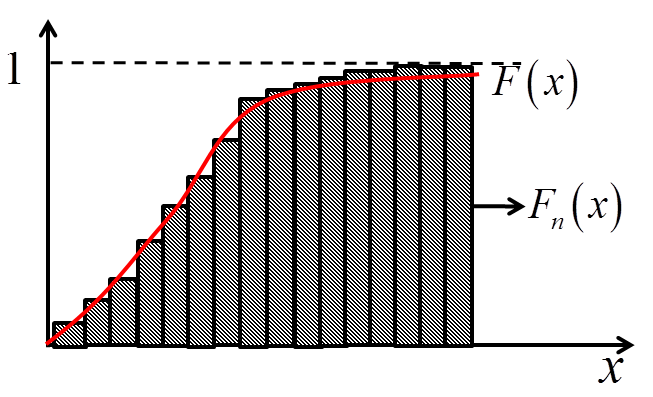
\includegraphics[height=3cm]{images/distribution_test.jpg}
            \caption{分布检验图}
            \label{fig:分布检验图}
            \end{figure}
            % \textcolor[rgb]{1 0 0}{todo:图片:分布检验图}\\
            将$F_n(x)$视为一个动态曲线,随着样本量$n$的变化而变化,这样有利于理解极限定理(局部相似和全局相似)。我们知道$F_n(x)$是一个统计量,是样本的函数,如果$F_n(x)$和$F(x)$的最大离差都很小,则我们就没有理由拒绝原假设。构建如下统计量
            \begin{align*}
            T \triangleq D_n = \sup_{-\infty <x <\infty}|F_n(x) - F(x)|
            \end{align*}
            \par
            下面,我们来研究一下检验统计量$D_n$的分布情况。关于统计量$D_n$,有格里汶科定理:
            \begin{align*}
            P \left( \lim\limits_{n\rightarrow \infty} D_n = 0 \right) = 1
            \end{align*}
            $D_n$几乎处处以概率1趋于0。Komogrov于1933年给出了$D_n$的精确分布
            \begin{align*}
            P \left( D_n \leqslant \lambda +\frac{1}{m} \right)  =
            \left\{
              \begin{aligned}
              &0 ,& \lambda \leqslant 0\\
              &\int_{\frac{1}{2n}-\lambda}^{\frac{1}{2n}+\lambda} \int_{\frac{3}{2n}-\lambda}^{\frac{3}{2n}+\lambda} \cdots\int_{\frac{2n-1}{2n}-\lambda}^{\frac{2n-1}{2n}+\lambda} n!\mathrm{d}y_1\mathrm{d}y_2\dots\mathrm{d}y_n ,& 0< \lambda \leqslant \frac{2n-1}{2n}\\
              &1 ,& \lambda >\frac{2n-1}{2n}
              \end{aligned}
            \right.
            \end{align*}
            \par
            $D_n$的渐近分布:当$n$较大时,上式就变得不易求解,在$n = 30$时,$D_n$渐近分布就和精确分布相似了。$D_n$的渐近分布为
            \begin{align*}
            P\{\sqrt{n}D_n<\lambda\} = \sum_{j=-\infty}^\infty (-1)^j e^{-2j^2\lambda^2} \quad j>0
            \end{align*}
            \par
            有了分布之后,我们就可以设置阈值$\alpha$,然后进行假设检验了。K-Stest的改进方向:上面提到过的KS检验需要有很高的要求,要求$H0$中的分布$F(x)$完全已知,不能有任何参数,如果含有未知参数,$F(x|\theta),\theta\in \Theta$,则量$D_n$就不再是统计量了,因为统计量只要求是样本的函数,而不能有外来参数$\theta$。如果我们用样本来估计参数$\theta$时,$D_n = \sup_x|F_n(x) - F(x|\hat{\theta})|$的分布是未知的,这使得检验难以进行。幸运的是,lillie于1967年提出用$\hat{\theta}$来代替$\theta$,然后再进行KS检验的lillie检验,值得注意的是,lillietest不适用与非位置尺度分布的检验。这里,我们直接给出其matlab命令,对其原理不做介绍。
            \par
            [h,p,kstat,crival] = lillietest(x,alpha,dister)\\
            其中:参数dister用于指定分布,参数值为'norm'时表示正态分布,'exp'表示指数分布,'ev'表示极值分布。其余参数和jbtest相似,不做说明。
        \subsubsection{卡方拟合优度检验}
            \par
            接下来介绍一个应用最为广泛的分布检验方法-$\chi^2$拟合优度检验。从检验的名字也可以看出该检验时如何进行的,$\chi^2$拟合优度检验和前面我们刚开始提到的检验有极大的相似性。$\chi^2$检验原本是为属性(分类)数据服务的,由于连续分布可以离散化,所以其对连续分布检验也同样适用,但要注意的是:窗宽$h$会严重影响检验结果。卡方拟合优度检验的原假设和最终的决策方法和之前介绍的方法相同,不同的是统计量的构造。对于统计量的构造\\
            \textbf{Step1}.将$x$的取值划分为几个区间段。设置$h$为窗宽(区间段长度),则有区间段数目为$\frac{Range(x)}{h}$(这里,我们假设Range(x)可以被$h$整除),$Range(x) = \max(x) - \min(x)$。对于外来参数$h$的确定,可以参考前面介绍的方法,也可以参考后面非参数统计部分核密度估计中$h$的确定方法。\\
            \textbf{Step2}.统计落入各区间段的样本数量$n_i$,这里的$n_i$是实际频数。如果$x_i$落在区间段边界上,我们采用“计上不计下”的原则来计数。\\
            \textbf{Step3}.计算落入各区间段的理论概率$p_i$和理论频数$np_i$。设第$i$个区间为$[a_{i-1},a_i]$,则
            \begin{align*}
            p_i = P\{a_{i-1} \leqslant x \leqslant a_i\} = F(a_i) - F(a_{i-1})
            \end{align*}
            并且,如果$F(x)$中包含参数$\theta$,则用样本先估计$\theta$,然后再计算理论概率。\\
            \textbf{Step4}.计算统计量。
            \begin{align*}
            T = \sum_{i=1}^{[Range(x)/h]} \frac{(n_i - np_i)^2}{np_i} \overset{\cdot}{\sim} \chi^2([Range(x)/h] - 1)
            \end{align*}
            如果$p_i$是估计值$\hat{p}_i$,则
            \begin{align*}
            T = \sum_{i=1}^{[Range(x)/h]} \frac{(n_i - n\hat{p}_i)^2}{n\hat{p}_i} \overset{\cdot}{\sim} \chi^2([Range(x)/h] - 1)
            \end{align*}
            \par
            $\chi^2$拟合优度检验的改进思路:卡方拟合优度检验的核心工作是样本密度$\hat{f}(x)$的计算(总体密度的估计)。在Step1中,我们硬性的将$x$划分了区间段,下面,我们换一种思路,在给定窗宽$h$后,我们不去统计落入$[a_{i-1},a_i]$的样本个数$n_i$,而是统计落入以$x_i$为中心的$[x_i-h/2,x_i+h/2]$的样本个数,然后再计算理论频数,由实际频数减去理论频数求平方后除理论频数,继续构建$\chi^2$统计量,只不过这里的自由度变为$(n-1)$。
            \par
            $\chi^2$拟合优度检验的matlab命令为
            \par
            [h,p,stats] = chi2gof(x,param,$\dots$)\\
            其中:参数'nbins'是组数;'ctrs'是组中点;'edges'是组边界;'cdf'的参数值可以是$\{@ normcdf,\mu,\sigma^2\}$;'nparm'分布中未知参数的个数;'emin'最小理论频数;'frequency'$x$中个元素出现个频数;'alpha'显著水平。
\section{非参数统计}
    \par
    前面介绍的估计和检验都是基于参数的,比如单总体均值估计,我们是假设总体服从正态分布,然后再估计正态分布的均值。这一部分,我们扔掉正态总体的前提,让数据自己说话。在前面的参数统计部分,我们讨论了单总体参数估计与检验、两总体均值估计与检验和多总体方差分析等问题。在非参数统计部分,我们仍然简单的介绍一下这些问题:单总体推断(估计)和检验、两总体位置尺度推断和检验以及多总体方差分析。
    \par
    前面介绍的许多方法都是基于正态总体的,如果我们对总体不是很了解,不能确定其是否为正态,或者经过分布检验后,确定总体分布不是正态,那么这些方法就失效了。现在的问题是:如果对总体分布不确定,或者总体不是正态分布,那么我们就不能估计均值、检验均值了吗?可以的,我们可以根据均值等统计数字特征的最原始定义和性质来进行估计和检验,比如:如果我们要检验总体的中位数$M_{0.5}$是否为$q_0$,可以依据中位数的原始定义和性质,将样本数据排序后,有一半样本在$q_0$左边,一半在$q_0$右边,那么我们就不能拒绝原假设。同样,我们可以检验总体的分位数。
    \subsection{单总体推断与检验}
        \subsubsection{符号检验}
            \par
            我们先来介绍用于中位数检验的符号检验方法\footnote{单总体中位数检验的R命令为binom.test。}。我们要检验总体的中位数$M_{0.5}$是否为$q_0$。\\
            \textbf{Step1}.首先设定原假设$H0:M_{0.5} = q_0$,备择假设$H1:M_{0.5} \neq q_0$。\\
            \textbf{Step2}.然后再来构建检验统计量,当$H0$成立的时候,样本应该有一半落在$q_0$左边,一半落在$q_0$的右边,即$x_i$落在$q_0$左边的概率为$\frac{1}{2}$,既然如此,我们可以记录一下落在$q_0$左右的数据量,记
            \begin{align*}
            s^+ = \sum I_{(x_i<q_0)}\\
            s^- = \sum I_{(x_i>q_0)}
            \end{align*}
            令$s= \min \{s^+,s^-\}$,有$s\sim b(n,q_0) \overset{L}{\sim}N(nq_0,nq_0(1-q_0))$。我们设定检验统计量为$T = s\sim b(n,q_0) $。\\
            \textbf{Step3}.最后我们来进行决策,我们可以根据p值进行决策,也可以设定显著水平$\alpha$。

        \subsubsection{Wilcoxon符号秩检验}
            \par
            在介绍Wilcoxon符号秩检验之前,我们先介绍一下样本秩的概念。我们给样本$x_i$秩$R_i$,比如有5个样本:$x_1 = 0.38,x_2 = 0.23,x_3 = 0.51,x_4 = 0.40,x_5 = 0.15$,那么,他们对应的秩为$R_1 = 3,R_2 = 2,R_3 = 5,R_4 = 4,R_5=1$。可以看出,$R$是一个统计量,$R_i$也是一个统计量,它标志着样本$x_i$在所有样本中的大小,其均值和方差为
            \begin{align*}
            &E(R_i) = \frac{n+1}{2} \\
            &Var(R_i) = \frac{n^2-1}{12}\\
            &Cov(R_i,R_j) = -\frac{n+1}{12}
            \end{align*}
            \par
            $R_i$只是$x_i$的一个得分,当然,这个得分可以定义成其他形式,比如我们在$R_i$外面套一层函数$a(R_i)$,示例:正态得分
            \begin{align*}
            a(r) = Z^{-1}\left\{ \frac{1}{2} + \frac{r}{2(n+1)} \right\}
            \end{align*}
            \textbf{Step1}.原假设$H0:$单峰分布$F(x)$的对称中心为$\theta$。\\
            \textbf{Step2}.构建统计量。前面构建的符号统计量$s$仅考虑了样本点的大小,而未考虑其绝对值大小,但其绝对值的大小有时候是很重要的,例如对样本$-0.21,-0.2,-0.13,-0.01,0,15,50,100,150$来说,$0$是中位数,正号负号数目一样,如果只看秩而不看数据,给人的印象是一个很对称的样本。但实际则不然,问题出来样本的绝对值大小没有考虑。假设样本为$x_1,\dots,x_n$,样本的顺序(统计量)为$x_{(1)},\dots,x_{(n)}$,样本绝对值(统计量)为$|x_1|,\dots,|x_n|$,样本绝对值的顺序统计量为$|x|_{(1)},\dots,|x|_{(n)}$,用$R_j^+$表示$|x_j|$在绝对值样本中的秩,则原假设成立的情况下,有
            \begin{align*}
            \sum I\{x_{i} > \theta \}\cdot R_i^+ = \sum I\{x_{i}<\theta\}R_i^+
            \end{align*}
            令$u_i = I\{x_{i} > \theta \}$,定义Wilcoxon符号秩统计量为
            \begin{align*}
            W^+ = \sum u_i\cdot R_i^+
            \end{align*}
            它是正的样本点按绝对值所得的秩的和。$W^+$不仅有样本的正负信息,而且还有样本的数值大小信息,和符号检验相似,我们在$W^+$较小的时候拒绝原假设,认为总体的对称中心不为$\theta$。关于检验统计量$W^+$的分布,可以参考《非参数统计》王星P75。在大样本下,$W^+$具有近似正态性
            \begin{align*}
            &E(W^+) = \frac{1}{2} \sum_{i=1}^n i =\frac{1}{4}n(n+1) \\
            &Var(W^+) = \frac{1}{4}\sum_{i=1}^n i^2 = \frac{1}{24}n(n+1)(2n+1)
            \end{align*}
            于是有
            \begin{align*}
            \frac{W^+ - E(W^+)}{\sqrt{W^+}} \xrightarrow{L} N(0,1) ,\quad n\rightarrow \infty
            \end{align*}
            \par
            上述证明可以参考《高等数理统计》P251。Wilcoxon符号秩检验的R程序为Wilcox.test。MATLAB用ranksum进行Wilcoxon秩和检验,用signtest做成对样本的符号检验,用signrank做成对样本的Wilcoxon符号秩检验。
    \subsection{两总体位置与尺度推断与检验}
        \par
        对独立两样本位置检验,可以使用Broon-Mood检验和Wilcoxon-Mann-whithey秩和检验,其R命令为wilcox.test(x,y,alt = "less")。对成对两样本位置检验,可以使用Wilcoxon检验,其R命令wilcoxon(x,y,paired = T,alt = "less")。对独立两样本尺度检验,可以使用Mood检验方法和Moses检验方法,在R包stats和fBsics有命令mood.test(x,y,alt = "greater")。
    \subsection{非参数方差分析}
        \subsubsection{单因素方差分析的K-S检验}
            \par
            Kruskal-Wallis检验用于单因素方差分析,要求样本量足够大,其原假设为$H0:k$个总体位置相同。其检验统计量为
            \begin{align*}
            H = \frac{12}{n(n+1)} \sum_{j = 1}^k \frac{R_{:j}^2}{n_j} - 3(n+1) \sim \chi^2(k+1)
            \end{align*}
            其中:$n$为样本总数,$k$为因素水平数,$R_{:j} = \sum_{i=1}^{n_j}R_{ij}$为第$j$组样本的秩和,$n_j$为第$j$组样本数。
            \par
            Kruskal-Wallis检验的R命令为kruskal.test,其MATLAB命令为
            \par
            [p,table,stats] = kruskalwallkis(x,group,displayopt)
        \subsubsection{双因素方差分析的Friedman检验}
            Friedman检验要求各总体分布的形式相同,位置参数可以不同。其原假设为$H0:\mu_i = \mu_j$,检验统计量为
            \begin{align*}
            Q = \frac{12}{nk(k+1)} \sum_{j=1}^kR_{:j}^2 - 3n(k+1) \sim \chi^2(k-1)
            \end{align*}
            其中:$n$为样本数,$k$为组数,$R_{:j}$为第$j$组样本的秩和。Friedman检验的R命令为friedman.test(y,groups,blocks),其MATLAB命令为
            \par
            [p,table,stats] = friedman(x,reps,displayopt)
            \par
            思考:对于同一个原假设,有不同的检验方法,那么如何评价各检验方法的功效呢?
\section{相关性分析}
    \subsection{相关性简介}
        \par
        相关性分析是统计分析的一个重点,前面我们分析的一般是单总体(单个变量)的估计与检验问题,在方差分析中分析了分类变量对连续变量的影响(两变量或多变量的相关性)。后面的内容我们要讨论变量相关性问题,比如:连续变量和连续变量的相关性、分类变量和连续变量的相关性、分类变量和分类变量的相关性、有序分类变量的相关性以及多变量之间的相关性。当然,相关性分析是具有一定假设和前提的,比如常见的Pearson相关性分析就要求变量是正态的,并且这种分析仅能检验两连续变量之间是否具有线性关系,如果变量之间是其它关系,Pearson就变得无能为力了。
        \par
        这里顺便说一下数据分析的一般流程。如果数据已经规整好了(结构化数据),我们的分析步骤一般是:1、设置变量属性和变量值标签,缺失值、异常值的处理。常见的变量属性为:连续变量、二分类变量、多分类变量以及有序变量,其实就是SPSS中的变量属性设置。变量值标签即为分类变量的变量值注释。2、变量的描述统计(均值、方差以及极大极小值等)。3、单总体(单变量)估计与检验。4、变量相关性检验。分类变量对连续变量的ANOVA,连续变量对连续变量的Pearson相关性以及Kendall秩相关分析(非参数),分类变量对分类变量的列联表分析,有序变量对有序变量的列联表分析和spearman秩、kendall秩相关分析。5、建模。设置目标变量,即$y$,$y$可以是一个变量也可以是多个变量,可以是连续变量也可以是分类变量,挑选自变量$x_1,x_2\dots$,建立变量关系模型$y = f(x)$。6、模型的检验与比较。关于定题和结论这里不介绍。下面,我们将介绍一些变量相关性检验的方法,在这一部分后面的章节中,我们将介绍变量关系模型:线性回归、SVM、RVM和神经网络ANN等。
    \subsection{连续变量对连续变量的相关性}
        \par
        首先,我们先来介绍用于连续变量相关性检验的Pearson积矩线性相关系数$\rho$、Kendall秩相关系数$\tau$和Spearman秩相关系数$\rho_s$。设我们现在要考虑变量$x$和$y$的关系,有样本数据$x_1,x_2,\dots,x_n$和$y_1,y_2,\dots,y_n$。
        \paragraph{Pearson相关系数}在变量$x,y$为正态总体的假设前提下,我们有$x,y$的Pearson线性相关系数
        \begin{align*}
        \hat{\rho} = \frac{\sum\limits_{i=1}^n(x_i-\bar{x})(y_i-\bar{y})}{\sqrt{\sum\limits_{i=1}^n(x_i-\bar{x})^2}\sqrt{\sum\limits_{i=1}^n(y_i-\bar{y})^2}}
        \end{align*}
        其中:$\bar{x} = \sum_{i=1}^nx_i,\bar{y} = \sum_{i=1}^ny_i$是极大似然估计,由极大似然估计得不变性,所以$\hat{\rho} $也是总体相关性的极大似然估计。关于极大似然估计的不变性,可以参考《数理统计学》。
        \paragraph{Kendall秩相关系数}是Maurice Kendall于1938年提出的方法,常用希腊字母$\tau$表示。设有两个随机变量$x,y$,$x,y$可以是(有序)分类变量也可以是连续变量,设样本量为$n$。定义$(x_i,y_i)$为一个样本对,样本对的一致性定义如下:
        \begin{definition}[样本对的一致性]
        当$x_i>x_j$并且$y_i>y_j$,或者$x_i<x_j$并且$y_i<y_j$,即$(x_i-x_j)(y_i-y_j)>0$,则称$x_i,y_i$一致;当$(x_i-x_j)(y_i-y_j)<0$,则称$x_i,y_i$不一致;当$(x_i-x_j)(y_i-y_j)=0$,称$x_i,y_i$既不是一致的也不是不一致。
        \end{definition}
        \par
        记$G$为样本中样本对一致的样本对数量,$H$为样本中样本对不一致的样本对数量,则Kendall秩相关系数的计算公式为
        \begin{align*}
        \tau = \frac{G-H}{\frac{1}{2}{n(n-1)}}
        \end{align*}
        \par
        注意:上述公式仅适用于样本$x,y$中不存在相同元素的情况。对于样本中存在相同元素的情况,比如:$x$的样本值为$1, 2, 3, 4, 3, 3, 2$,我们就需要对Kendall计算公式进行修正,修正计算公式为
        \begin{align*}
        \tau' = \frac{G-H}{\sqrt{(n_3-n_1)(n_3-n_2)}}
        \end{align*}
        其中:
        \begin{align*}
        &n_3= \frac{1}{2}n(n+1)\\
        &n_1 = \sum_{i=1}^s\frac{1}{2}u_i(u_i-1)\\
        &n_2 = \sum_{i=1}^t\frac{1}{2}v_i(v_i-1)
        \end{align*}
        对于上面的$s,t$的计算,以$s$为例,将$x$中的相同元素分别组合成小集合,$s$表示集合$x$中拥有的小集合数,例如$x$包含元素$1, 2, 3, 4, 3, 3, 2$,那么这里得到的$s$则为2,因为只有2和3有相同元素,$u_i$表示第$i$个小集合所包含的元素个数。

        \paragraph{Spearman秩相关系数}属于非参数方法,从其名称中也可以看出它是一种基于秩的方法。其定义为
        \begin{align*}
        \hat{\rho}_s = \frac{\sum\limits_{i=1}^n(R_i - \bar{R})(Q_i - \bar{Q})}{\sqrt{(R_i - \bar{R})^2}\sqrt{(Q_i - \bar{Q})^2}}
        \end{align*}
        其中:
        \begin{align*}
        &\bar{R} = \frac{1}{n}\sum_{i=1}^nR_i\\
        &\bar{Q} = \frac{1}{n}\sum_{i=1}^nQ_i
        \end{align*}
        由于
        \begin{align*}
        &\sum_{i=1}^n R_i = \sum_{i=1}^n Q_i = \frac{n(n+1)}{2}\\
        &\sum_{i=1}^n R_i^2 = \sum_{i=1}^n Q_i^2 = \frac{n(n+1)(2n+1)}{6}
        \end{align*}
        所以,Spearman秩相关系数也可以写为
        \begin{align*}
        \hat{\rho}_s = 1-\frac{6}{n(n^2-1)}\sum_{i=1}^n(R_i-Q_i)^2
        \end{align*}
        可以发现,Spearman秩方法和Pearson方法很相似。上面介绍的三种相关性度量方法中,后两种属于非参数统计方法,第一种是参数统计方法。MATLAB中的命令为
        \par
        coeff = corr(x,y,'type','Kendall')\\
        其中:参数'type'指定了相关系数的类型,其参数值可以是'Pearson'、'Spearman'和'Kendall'。
        \paragraph{互信息}是信息论中的概念,这个概念我们在后面还会用到。Shannon于1948年首次定义了互信息(mutual information),用于度量两个变量间的相互依赖程度,其定义为
        \begin{align*}
        I(x,y) = \iint p(x,y) \log \left( \frac{p(x,y)}{p(x)p(y)} \right)  \mathrm{d}x\mathrm{d}y
        \end{align*}
        其中:$p(x,y)$为联合概率密度,$p(x),p(y)$为边际密度,$\log$的底数可以取2、10、$e$或者其它。互信息的样本估计为
        \begin{align*}
        I(x,y) = \sum_i \sum_j p(x_i,y_j) \log \left( \frac{p(x_i,y_j)}{p(x_i)p(y_j)} \right)
        \end{align*}

        \par
        由于总体概率密度未知,所以我们一般才用样本的概率密度来替代总体的密度,相应的样本密度计算方法可以采用非参数统计中的核密度估计和K邻近距离KNN。
        \paragraph{距离相关性}是Szkely于2007年提出的一种相关性方法,设$X$是$p$维随机向量,$Y$是$q$维随机向量,$X,Y$具有有限1阶矩。定义$X,Y$总体距离协方差为
        \begin{align*}
        V(X,Y) = \sqrt{V^2(X,Y)} &= \sqrt{||f_{X,Y}(t,s) - f_{x}(t)f_{Y}(s)||^2}\\
        &= \sqrt{\frac{1}{C_pC_q }\int \frac{|f_{X,Y}(t,s) - f_{x}(t)f_{Y}(s)|^2}{|t|_p^{1+p}|s|_q^{1+q}}\mathrm{d}t\mathrm{d}s}
        \end{align*}
        其中:$f_X(t)$是$X$的特征函数,$f_{XY}(t,s)$是$X,Y$的联合特征函数,
        \begin{align*}
        C_d = \frac{\pi^{1+\frac{d}{2}}}{\Gamma \left( \frac{1+d}{2} \right) } ,\quad d = p \ or\ q
        \end{align*}
        总体距离方差为
        \begin{align*}
         V(X,X) = \sqrt{V^2(X,X)} &= \sqrt{||f_{X,X}(t,s) - f_{x}(t)f_{X}(s)||^2}
        \end{align*}
        总体距离相关性为
        \begin{align*}
        R(X,Y) = \sqrt{R^2(X,Y)}=
        \left\{
            \begin{aligned}
            \sqrt{\frac{V^2(X,Y)}{\sqrt{V^2(X)V^2(Y)}}}\quad V^2(X)V^2(Y)>0\\
            0\quad V^2(X)V^2(Y)<0
            \end{aligned}
        \right.
        \end{align*}
        \paragraph{MIC相关性}是哈佛大学Broad研究院的Reshef在2011年提出的一种数据相关性挖掘方法,MIC是maximal information Coefficient的缩写,其R命令在R包minerva中,命令为
        \par
        mine(x,y,master,alpha,C,n.cores,varthr)\\
        其中:x,y指定了数据集,alpha为网格分割的大小$B(n) = n_\alpha$ ,C为起点,n.cores是并行计算,varthr是新的样本最小方差。
        \par
        考虑$x,y$两个变量,样本容量为$n$。MIC算法主要由以下2个因素决定:1、网格划分数,即在给定的数据集形成的散点图上,在$x$轴和$y$轴上分别进行多少次的划分;2、网格划分的位置,即如果在$x$轴上划分$n_x$次,那么这$n_x$个划分点是等距放置还是以某种其他方式放置在$x$轴上?若给定划分数和划分位置,则给定了一种划分,计算该划分下的互信息值
        \begin{align*}
        I(x,y) = \iint p(x,y) \log \left( \frac{p(x,y)}{p(x)p(y)} \right) \mathrm{d}x\mathrm{d}y
        \end{align*}
        其中:$p(x,y)$用落入格子中的样本频率来估计,$p(x),p(y)$用落入$(k,k+1)$和$(l,l+1)$区间的样本频率估计($0 \leqslant k \leqslant n_x-1, 0 \leqslant l \leqslant n_y-1$),$n_x,n_y$为$x,y$轴划分段数。
        \par
        如果固定网格划分数为$n_x,n_y$,则通过改变网格划分位置,会得到不同的互信息值,记其中最大的互信息值为$I_{n_x\times n_y}(x,y)$。进一步,为了方便在不同维度下进行比较,将其标准化,使其取值在$[0,1]$
        \begin{align*}
        M_{n_x\times n_y}(x,y) = \frac{I_{n_x\times n_y}(x,y)}{\log (\min\{x,y\})}
        \end{align*}
        设定网格划分数目的上限$B(n)$,则最大互信息MIC定义为
        \begin{align*}
        MIC(x,y) = \max_{n_x \times  n_y <B(n)} \{M_{n_x\times n_y}(x,y)\}
        \end{align*}

    \subsection{分类变量对分类变量的相关性}
        \par
        上面介绍了几种用于处理连续变量相关性的方法,下面,我们来处理分类变量相关性问题。
        \subsubsection{四格表}
            \par
            四格表即$2\times 2$列联表,用于处理变量$A,B$皆是二分类变量的情况。四格表一般形式如表(\ref{tab:四格表})所示
            \begin{table}[H]
            \caption{四格表}
            \label{tab:四格表}
            \centering
            \begin{tabular}{c|cc|c}
            {}& B& $\bar{B}$ & {}\\
            \hline
            A& $n_{11}$& $n_{12}$ & $n_{1+}$\\
            $\bar{A}$& $n_{21}$& $n_{22}$ & $n_{2+}$\\
            \hline
            {}& $n_{+1}$& $n_{+2}$ & $n$\\
            \end{tabular}
            \end{table}
            % \textcolor[rgb]{1 0 0}{todo:表格:四格表}\\
            例如:$A$表示是否吸烟,$B$表示是否得肺癌。表中的$A$表示吸烟,$\bar{A}$表示不吸烟,$A$行$B$列的格$n_{11}$表示吸烟得肺癌的人数,$n_{1+}$表示吸烟的人数,$n$为总样本数,$n = n_{1+}+n_{2+}= n_{+1}+n_{+2}$。我们一般默认把原因变量“吸烟”作为行,把结果变量(被影响)“肺癌”作为列。
            \par
            下面,我们主要说明完全随机四格表,即$n_{11},n_{12},n_{21},n_{22}$都是随机变量。首先,要说明的是,对四格表而言,不相关和独立是等价的,其证明可参考《属性数据分析》王静龙P45。假设$n_{ij}$服从泊松分布$n_{ij}\sim p(\lambda_{ij})$
            \begin{theorem}
            若$n_{ij}\sim p(\lambda_{ij})$,并且相互独立,则在$n = n_{11}+n_{12}+n_{21}+n_{22}$给定后,$(n_{11},n_{12},n_{21},n_{22})$的条件分布为多项分布
            \begin{align*}
            (n_{11},n_{12},n_{21},n_{22}) = M(n,p_{11},p_{12},p_{21},p_{22})
            \end{align*}
            其中:
            \begin{align*}
            p_{ij} = \frac{\lambda_{ij}}{\sum_{ij}\lambda_{ij}}
            \end{align*}
            \end{theorem}
            \begin{Proof}
            由泊松分布的可加性,有
            \begin{align*}
            n\sim p(\lambda_{11}+\lambda_{12}+\lambda_{21}+\lambda_{22})
            \end{align*}
            所以,当$n$给定后,$(n_{11},n_{12},n_{21},n_{22})$的条件分布为
            \begin{align*}
            &\frac{\left( \frac{\lambda_{11}^{n_{11}}}{n_{11}} e^{-\lambda_{11}} \right)
            \left( \frac{\lambda_{12}^{n_{12}}}{n_{12}} e^{-\lambda_{12}} \right)
            \left( \frac{\lambda_{21}^{n_{21}}}{n_{21}} e^{-\lambda_{21}} \right)
            \left( \frac{\lambda_{22}^{n_{22}}}{n_{22}} e^{-\lambda_{22}} \right)}{\frac{(\sum_{ij}\lambda_{ij})^n}{n!}e^{-\sum_{ij}\lambda_{ij}}}\\
            ={}&\frac{n!}{n_{11}!n_{12}!n_{21}!n_{22}!}p_{11}^{n_{11}}p_{12}^{n_{12}}p_{21}^{n_{21}}p_{22}^{n_{22}}
            \end{align*}
            \end{Proof}
            \par
            由于四格表的独立性和不相关等价,所以四格表的独立性检验($A,B$之间不相关)的原假设为
            \begin{align*}
            H0:p_{ij} = p_{i+}p_{+j}\quad \forall ij\in \{1,2\}\\
            H1:p_{ij} \neq p_{i+}p_{+j}\quad \exists ij\in \{1,2\}
            \end{align*}
            \par
            接下来的问题就是构建检验统计量,下面我们介绍两种检验统计量:1、卡方检验统计量2、似然比检验统计量。
            \par
            (1)构建卡方统计量
            \begin{align*}
            T =\sum_{i=1}^2\sum_{j=1}^2\frac{(n_{ij} - n{p}_{ij})^2}{n{p}_{ij}}
            \end{align*}
            其中:$n_{ij}$为实际频数,$n{p}_{ij}$为期望频数。由于当然,总体的$p_{ij}$未知,所以用样本估计$\hat{p}_{ij}$,于是统计量变为
            \begin{align*}
            T =\sum_{i=1}^2\sum_{j=1}^2\frac{(n_{ij} - n\hat{p}_{ij})^2}{n\hat{p}_{ij}}
            \end{align*}
            \par
            下面讨论总体概率$p_{ij}$的估计$\hat{p}_{ij}$。在$H0$中,我们假设$p_{ij} = p_{i+}p_{+j}$,而总体概率$p_{1+},p_{2+},p_{+1},p_{+2}$的极大似然估计(频率估计)为
            \begin{align*}
            \hat{p}_{1+} = \frac{n_{1+}}{n},\hat{p}_{2+} = \frac{n_{2+}}{n},\hat{p}_{+1} = \frac{n_{+1}}{n},\hat{p}_{+2} = \frac{n_{+2}}{n}
            \end{align*}
            所以,$\hat{p}_{ij}$为
            \begin{align*}
            \hat{p}_{ij} = \hat{p}_{i+}\hat{p}_{+j} = \frac{n_{i+}n_{+j}}{n^2}
            \end{align*}
            于是检验统计量变为
            \begin{align*}
            T &=\sum_{i=1}^2\sum_{j=1}^2\frac{(n_{ij} - n\hat{p}_{ij})^2}{n\hat{p}_{ij}}\\
            &=\sum_{i=1}^2\sum_{j=1}^2\frac{\left(n_{ij} - \frac{n_{i+}n_{+j}}{n}\right)^2}{\frac{n_{i+}n_{+j}}{n}}\\
            &=\sum_{i=1}^2\sum_{j=1}^2 \frac{n_{ij}^2}{\frac{n_{i+}n_{+j}}{n}} - n\\
            &=\frac{n(n_{11}n_{22} - n_{12}n_{21})}{n_{1+}n_{2+}n_{+1}n_{+2}}
            \end{align*}
            和前面分布估计中的卡方拟合优度检验一样,检验统计量$T$服从卡方分布,并且,由于$p_{1+}+p_{2+} = p_{+1}+p_{+2} = 1$,所以未知参数只有2个,卡方分布的自由度为$df = 4-1-2$,即
            \begin{align*}
            T \overset{\cdot}{\sim} \chi^2(1)
            \end{align*}
            \par
            经过连续性修正的检验统计量为
            \begin{align*}
            T' = \frac{n\left(|n_{11}n_{22} - n_{12}n_{21}|-\frac n2\right)}{n_{1+}n_{2+}n_{+1}n_{+2}}
            \end{align*}
            \par
            (2)构建似然比检验统计量
            \begin{align*}
            -2\ln (\varLambda) = -2\sum_{i=1}^2\sum_{j=1}^2n_{ij}\ln \left( \frac{\hat{p}_{ij}}{n_{ij}/n} \right)
            \end{align*}
            由
            \begin{align*}
            \hat{p}_{ij} = \frac{n_{i+}n_{+j}}{n^2}
            \end{align*}
            于是似然比检验统计量写为
            \begin{align*}
            -2\ln (\varLambda) = -2\sum_{i=1}^2\sum_{j=1}^2n_{ij}\ln \left( \frac{n_{i+}n_{+j}}{n_{ij}n} \right) \overset{\cdot}{\sim}\chi^2(1)
            \end{align*}
        \subsubsection{二维列联表}
            \par
            前面介绍的四格表是用于处理分类变量$A,B$是二分类的情况,仿照其表格结构,我们可以处理$A$是二分类变量$B$是多分类的情况,同样也可以处理$A,B$皆是多分类变量的情况。设有多分类变量$A,B$,$A$有$r$个水平,$B$有$c$个水平,其形成的二维列联表如表\ref{tab:二维列联表}所示
            \begin{table}[H]
            \caption{二维列联表}
            \label{tab:二维列联表}
            \centering
            \begin {tabular}{c|cccc|c}
            {}& $B_1$& $B_2$ & $\cdots$ &$B_c$ & {}\\
            \hline
            $A_1$& — &  —  & — & — & — \\
            $A_2$& — & $n_{22}$ & — & —&  — \\
            $\vdots $& — &  —  & — & — &$n_{i+}$\\
            $A_r$& — &  —  & — & — & — \\
            \hline
            {}& — &  —  & $n_{+j}$ & — & — \\
            \end{tabular}
            \end{table}
            % \textcolor[rgb]{1 0 0}{todo:表格:二维列联表}\\
            表中$A_i$表示变量$A$的第$i$个水平,$n_{ij}$表示是$A_i$和$B_j$的频数,$n_{i+}$是$A_i$的样本数量,$n$为总的样本数量,$p_{ij}$是$A_i$和$B_j$的概率(理论),$\hat{p}_{ij}$是$p_{ij}$的样本估计。
            \par
            现在,我们要检验变量$A,B$是否相关。我们设置原假设为$H0:\forall i\in r,j\in c,p_{ij} = p_{i+}p_{+j}$,即变量$A,B$相互独立,$P\{A_i \wedge  B_j\} = P(A_i)P(B_j)$。下面我们来构建检验统计量,我们有实际频数$n_{ij}$,其期望频数为$n{p}_{ij}$,可以构建卡方统计量
            \begin{align*}
            T = \sum_{i=1}^r\sum_{j=1}^c \frac{(n_{ij} - np_{ij})^2}{np_{ij}}
            \end{align*}
            但是,一般情况下$p_{ij}$是未知的,所以我们要用样本来估计之。设其样本估计量为$\hat{p}_{ij}$,于是期望频数为$n\hat{p}_{ij}$,卡方统计量$T$变为
            \begin{align*}
            T = \sum_{i=1}^r\sum_{j=1}^c \frac{(n_{ij} - n\hat{p}_{ij})^2}{n\hat{p}_{ij}}
            \end{align*}
            \par
            接下来讨论$\hat{p}_{ij}$的计算。由原假设$H0:p_{ij} = p_{i+}p_{+j}$,所以,$\hat{p}_{ij} = \hat{p}_{i+}\hat{p}_{+j}$,而$\hat{p}_{i+} = \frac{n_{i+}}{n},\hat{p}_{+j} = \frac{n_{+j}}{n}$,所以,期望频数为
            \begin{align*}
            np_{ij} \approx n\hat{p}_{ij} &= n\hat{p}_{i+}\hat{p}_{+j} \\
            &= n\frac{n_{i+}}{n}\frac{n_{+j}}{n} \\
            &=\frac{n_{i+}n_{+j}}{n}
            \end{align*}
            卡方统计量$T$变为
            \begin{align*}
            T &= \sum_{i=1}^r\sum_{j=1}^c \frac{(n_{ij} - n\hat{p}_{ij})^2}{n\hat{p}_{ij}}\\
            &=\sum_{i=1}^r\sum_{j=1}^c \frac{n_{ij}^2}{n_{i+}n_{+j}/n} -n \\
            &\sim \chi^2((r-1)(c-1))
            \end{align*}
            我们还可以构建如下似然比统计量
            \begin{align*}
            -2\ln \varLambda & = -2\sum_{i=1}^r\sum_{j=1}^cn_{ij}\ln \left( \frac{\hat{p}_{ij}}{n_{ij}/n} \right)  \\
            &=-2\sum_{i=1}^r\sum_{j=1}^cn_{ij}\ln \left( \frac{n_{i+}n_{+j}}{n_{ij}n} \right)
            \end{align*}
            \par
            上面介绍的四格表或者二维列联表仅用于检验两个变量$x,y$是否具有相关性,并没有给出$x,y$是正相关还是负相关,也没有给出相关性强度。对于$x,y$的正负相关性及相关性强度的检验,我们可以参考两连续随机变量相关性的Pearson相关性、Spearman相关性和Kendall相关性。在分类变量中,我们考虑如下相关性(相合性)问题:随着抑郁程度的增加,自杀倾向是否增加?即自杀倾向是否和抑郁程度成正比?设自杀倾向为$y$,抑郁程度为$x$,我们将自杀倾向和抑郁程度分为3个等级:$1,2,3$,标签为低中高。设样本数为$n$,抽取样本,可构建如表(\ref{tab:顺序变量列联表})形式的列联表
            \begin{table}[H]
            \caption{顺序变量列联表}
            \label{tab:顺序变量列联表}
            \centering
            \begin {tabular}{c|ccc}
            {} & 1 & 2 & 3 \\\hline
            1 & 195 & 93 & 34 \\
            2 & 20 & 27 & 27 \\
            3 & 26 & 37 & 39 \\
            \end{tabular}
            \end{table}
            % \textcolor[rgb]{1 0 0}{todo:表格:顺序变量列联表}\\
            \par
            对于$x,y$的相关性,我们可以采用前面介绍的Kendall相关性
            \begin{align*}
            \tau = \frac{2}{n(n+1)}Z
            \end{align*}
            其中:$Z = G-H$,$G$为样本中中一致序列的样本对数量,$H$为不一致的数量
            \begin{align*}
            Z = \sum_{1 \leqslant i<j \leqslant n} \mathrm{sign}((x_i-x_j)(y_i-y_j)) = G-H
            \end{align*}
            \par
            不过,在列联表中,我们需要进行一些修改。Kendall相关系数$\tau$修改为
            \begin{align*}
            \tau = \frac{Z}{\sqrt{[n(n-1)/2-T_A][n(n+1)/2-T_B]}}
            \end{align*}
            其中:$T_A,T_B$为
            \begin{align*}
            T_A = \sum_{i=1}^r \binom{n_{i+}}{2} = \sum_{i=1}^r\frac{n_{i+}(n_{i+}-1)}{2}\\
            T_B = \sum_{j=1}^c \binom{n_{+j}}{2} = \sum_{j=1}^c\frac{n_{+j}(n_{+j}-1)}{2}
            \end{align*}
            $Z = G-H$,列联表中$G,H$可以写为
            \begin{align*}
            G = \sum_{i=1}^{r-1}\sum_{j=1}^{c-1} n_{ij} \left( \sum_{k=i+1}^r\sum_{t=j+1}^c n_{kt}\right)  = \sum_{i<k}\sum_{j<t}n_{ij}n_{kt}\\
            H = \sum_{i=1}^{r-1}\sum_{j=1}^{c-1} n_{ij} \left( \sum_{k=i+1}^r\sum_{t=j+1}^{j-1} n_{kt}\right)  = \sum_{i<k}\sum_{j>t}n_{ij}n_{kt}
            \end{align*}
            \par
            我们还可以用Gamma系数$\gamma$和Somers系数$d$来衡量$x,y$相关性强弱。Gamma系数的计算公式为
            \begin{align*}
            \gamma = \frac{G-H}{G+H}
            \end{align*}
            Somers系数只使用与$2\times c$列联表,其计算公式为
            \begin{align*}
            d_{y|x} = \frac{G-H}{n(n-1)/2 - T_A}\\
            d_{x|y} = \frac{G-H}{n(n-1)/2 - T_B}
            \end{align*}
            \par
            上面介绍的相关性方法都是用来衡量$x,y$之间正负相关性强弱的(估计),并没有涉及到假设检验技术。对于相关性检验问题,可以参考《属性数据分析》王静龙P92。书中说的是:先计算$\tau$,或者$\gamma,d_{x|y},d_{y|x}$以及它们的标准误se(*),然后在原假设($H0:x,y$相互独立)成立时,检验统计量$T = \tau/\mathrm{se}(\tau)$的渐近服从标准正态分布。上面介绍的相关性度量和检验都是针对两个分类变量而言,可以尝试将其推广到多个分类变量。还可以考虑有缺失数据的情况,或者小样本的情况。
            \par
            MATLAB中用crosstab来实现列联表分析,其命令为
            \par
            [table,chi2,p,labels] = crosstab(x1,...,xn)\\
            其中:table即为列联表,chi2为卡方统计量值,p为p值,labels为标签和标签值,是一个元胞数组。R中的列联表有多种实现方式(毕竟R是专业统计工具嘛)。
            \begin{enumerate}
            \item table(var1,var2,$\dots$,varN):使用N个分类变量(因子)创建一个N维列联表。
            \item xtabs(formula,data):根据一个公式和一个矩阵或数据框创建一个N维列联表。
            \item prop.table(table,margins):依margins定义的边际列表将表中条目表示为分数形式。
            \item margin.table(table,margins):依margins定义的边际列表计算表中条目的和。
            \item addmargins(table,margins):将概述边margins(默认是求和结果)放入表中。
            \item ftable(table):创建一个紧凑的“平铺”式列联表
            \end{enumerate}
            \par
            table函数生成的结果对象类型为“table”,可以直接作为chisq.test等函数的参数输入,进行检验等。在计算列联表的时候,一般都希望可以同时获得行、列和总和范围内的百分比,而默认安装的R没有内置的给出这个功能的函数,不过还是提供了margin.table和prop.table分别解决这个问题。代码示例
            \begin{lstlisting}[language = R]
            #table创建列联表
            mytable2 <- table(A, B) #A是行变量,B是列变量
            #xtab创建列联表
            xtab(A ~ B, data=mydata, chisq = TRUE)
            #或者
            mytable3 <- xtabs(~A + B, data=mydata , chisq = TRUE) #mydata为一矩阵,需要交叉分类的变量放在"~"右侧,以"+"作为分隔符
            #margin.table()和prop.table()函数分别生成边际频数和比例。
            margin.table(mytable2,1) #1指的是第1个变量
            prop.table(mytable3,,2) #2指的是第2个变量
            prop.table(mytable3) #各单元格所占的比例
            #addmargins()函数为这些表格添加边际和
            addmargins(mytable2) #行与列分别相加
            addmargins(prop.table(mytable2)) #行与列分别相加
            #使用gmodels包中的CrossTable()函数是创建出类似于SAS的表格:
            library(gmodels)
            CrossTable(Arthritis$Treatment, Arthritis$Improved)
            #高维列联表
            mytable4 <- xtabs(~Treatment + Sex + Improved, data = Arthritis)
            ftable(mytable4) #将mytable4三维列联表转化为扁平形式
            margin.table(mytable4,1) #对第1个变量(Treatment)求和
            margin.table(mytable4,c(1,3)) #对第1个变量(Treatment)与第3个变量(Improved)作边际频数
            ftable(addmargins(prop.table(mytable4,c(1,2)),3))
            \end{lstlisting}

    \subsection{Copula}
        \subsubsection{Copula简介}
            \par
            从随机变量的独立性入手。如果两个随机变量$x,y$独立,则其联合概率密度$f(x,y)$等于各自边缘概率密度$f(x),f(y)$的乘积,即$f(x,y) = f(x)f(y)$。现在考虑,如果我们有了$f(x,y),f(x),f(y)$,那么,在$f(x,y)$中去掉$f(x),f(y)$,剩下的量是否就可以用来表示$x,y$之间的相关性?这种思想可以追溯到1959年Sklar提出的Copula函数。Sklar的理论是:联合概率密度可以分解为边缘密度函数和一个Copula函数,\underline{并且Copula函数唯一。}
            \par
            我们先来统一符号:$f$表示密度函数;$F$表示分布函数;$\theta$是参数;$C$是Copula函数;$x,y$是随机变量,$\mathbf{x}$是随机向量。
            \par
            Copula在法语中是链接交换的意思。Copula模型用来研究多变量相关性和求解联合密度(分布)的模型。多变量联合密度的求解一直是统计学中的难题,它不像一元变量有正态分布、均匀分布、指数分布以及各种分布族。我们后面讨论的Copula函数隶属于参数统计,但其多变的参数估计方法又不局限于参数方法。下面,我们先来简单介绍一下Copula,然后讨论Copula建模步骤。
            \par
            注:现代金融分析中,组合投资和资产定价都离不开资产相关性的度量。在后面的建模章节中,我们简单的讨论了关于股票的组合投资策略,其关键点就是收益率序列的建模及Copula-VaR相关性度量。
            \begin{definition}[Copula函数的定义]
            Copula是一个多元分布函数,其边缘分布是定义在$[0,1]$上的均匀分布,即$U(0,1)$,常用$C$表示,并且满足一下三个条件
            1). $C:[0,1]^n\rightarrow [0,1]$;
            2). $C$是有grounded的递增函数;
            3). $C$的所有边缘分布函数$C_i$满足:$C_i = C(1,\dots,1,u,1,\dots,1) = u,u\in [0,1],i = 1,\dots,n$。
            \end{definition}
            \par
            设$F_1,\dots,F_n$是随机变量$x_1,\dots,x_n$的分布函数,则$C[F_1(x_1),\dots,F_n(x_n)]$是表示已多变量的分布函数,其边缘分布函数就为$F_1,\dots,F_n$。由此可见Copula吧一些边缘分布链接为一个联合分布函数。
            \begin{theorem}[Sklar定理]
            设有$n$个随机变量$x_1,\dots,x_n$。若$F(x_1,\dots,x_n)$是$n$个随机变量的联合分布函数,其边缘分布为$F_1,\dots,F_n$,那么一定存在一个Copula函数$C$,使得
            \begin{align*}
            F(x_1,\dots,x_n) = C[F_1(x_1),\dots,F_n(x_n)]
            \end{align*}
            并且,如果边缘分布是连续的,那么Copula函数形式唯一。
            \end{theorem}
            \par
            利用上面的定理,我们可以将一个多维分布函数拆分成边缘分布函数组合的形式
            \begin{align*}
            f(x_1,\dots,x_n) &= \frac{\partial F(x_1,\dots,F_n)}{\partial x_1\dots,\partial x_n}\\
            &=\frac{\partial C[F_1(x_1),\dots,F_n(x_n)]}{\partial x_1\dots,\partial x_n}\\
            &=\frac{\partial C(u_1,\dots,u_n)}{\partial u_1\dots,\partial u_n}  \times \prod_i \frac{\partial F_i(x_i)}{\partial x_i}\\
            &=c(u_1,\dots,u_n) \times \prod_i f_i(x_i)\\
            &=c(\tilde{u}) \times \prod_i f_i(x_i)
            \end{align*}
            其中:$f(x_1,\dots,x_n)$为联合概率密度函数;$u_i = F_i(x_i),i = 1\dots,n$;$\tilde{u} = (u_1,\dots,u_n)$;$c(\tilde{u})$为Copula的密度函数。
            \par
            也就是说,我们可以将联合概率密度$f(\cdot)$拆分为两部分,前部分$c(\tilde{u})$为Copula的密度函数,表示变量$x_1,\dots,x_n$的相关性;后部分为边缘概率密度的乘积。当各变量相互独立时,$C(u_1,\dots,u_n) = u_1\times \dots \times u_n$。
            \par
            上面给出了Copula函数的定义,下面给出它的性质。Copula函数有许多优良的性质,比如:1、在利用Copula构建多维随机变量的联合分布$F$时,不需要对边缘分布$F_i(x_i)$作任何假设。2、Copula函数导出的相关性度量在严格单调增的变换下都不改变,有如下不变性定理
            \begin{theorem}[Copula不变性]
            (Nelsen.2006.)就两变量而言,对随机变量$x,y$做严格单调增变换$x^* = h_1(x),y^* = h_2(y)$,相应的Copula函数不变,即
            \begin{align*}
            C[F_1(x),F_2(y)] = C[F_1(x^*),F_2(y^*)]
            \end{align*}
            简写为$C_{xy} = C_{x^*y^*}$。
            \end{theorem}
            \par
            前面介绍的Spearman秩相关系数$\rho_s$和Kendall秩相关系数$\tau$都可以用Copula函数表示
            \begin{align*}
            &\rho_s(x,y) = 12\iint_{[0,1]^2}u_1u_2\mathrm{d}C(u_1,u_2) - 3\\
            &\tau(x,y) = 4 \iint_{[0,1]^2}C(u_1,u_2)\mathrm{d}C(u_1,u_2) - 1
            \end{align*}
            \par
            尾部相关性的Copula表示。在金融风险分析中,随机变量的尾部相关性是相当重要的。设$X,Y$为两个随机变量,条件概率$P\{X_1>x_1|X_2>x_2\}$反应了股票市场中一种股票涨高时,引起另一种股票涨高的概率。
            \begin{definition}[尾部相关性]
            设$X,Y$的分布函数为$F,G$,$X,Y$的上端尾部相关性和下端尾部相关性定义为
            \begin{align*}
            \lambda_u = \lim_{\alpha\rightarrow 1-}P\{Y>G^{-1}(\alpha)|X>F^{-1}(\alpha )\}\\
            \lambda_l = \lim_{\alpha\rightarrow 0+}P\{Y \leqslant G^{-1}(\alpha)|X \leqslant F^{-1}(\alpha )\}
            \end{align*}
            其中:$F^{-1}(\alpha) = \inf(x|X \geqslant \alpha)$,$G^{-1}(\alpha) = \inf(y|Y \geqslant \alpha)$。
            \end{definition}
            \par
            如果$\lambda_u$(或$\lambda_l$)存在且$\lambda_u \in [0,1]$,那么$X,Y$具有渐近上(下)端尾部相关性,如果$\lambda _u = 0$,则$X,Y$在上(下)端尾部独立。尾部相关系数的Copula表示形式为
            \begin{align*}
            \lambda _u = \lim_{\alpha\rightarrow1-}\frac{\bar{C}(\alpha,\alpha)}{1-\alpha}
            \end{align*}
            其中:$\bar{C}(u,u) = 1-2u+C(u,u)$。推导如下:
            \begin{align*}
            \lambda_u &= \lim_{\alpha\rightarrow 1-}P\{Y>G^{-1}(\alpha)|X>F^{-1}(\alpha )\}\\
            &= \lim _{\alpha\rightarrow 1-} \frac{P\{Y>G^{-1}(\alpha),X>F^{-1}(\alpha)\}}{P\{X>F^{-1}(\alpha)\}}\\
            &=\lim _{\alpha\rightarrow 1-}\frac{1-P\{Y \leqslant G^{-1}(\alpha)\} - P\{X \leqslant F^{-1}(\alpha) \} + P\{Y \leqslant G^{-1}(\alpha),X \leqslant F^{-1}(\alpha) \}  }{1 - P\{X \leqslant F^{-1}(\alpha) \} }\\
            &=\lim _{\alpha\rightarrow 1-}\frac{1-2\alpha+C(\alpha,\alpha)}{1-\alpha}
            \end{align*}
            \par
            不同类型的阿基米德Copula族对尾部相关性的刻画是不一样的,Gumbel Copula和Clayton Copula具有非对称性,可以用来描述变量间非对称的相关模式,不同的是Gumbel Copula强调随机变量间具有更高的上端尾部相关性,而Clayton Copula则强调随机变量间具有更高的下端尾部相关性,Frank Copula则更高强调分布尾部相关性的变化,在其分布的上尾和下尾,变量间的相关性是对称增长的。

        \subsubsection{一些Copula函数}
            \par
            (1)二元正态Copula函数
            \begin{align*}
            C(u,v|\rho) = \int_{-\infty}^{\varPhi^{-1}(u)} \int_{-\infty}^{\varPhi^{-1}(v)} \frac{1}{2\pi \sqrt{1-\rho^2}} \exp\left\{ -\frac{s^2-2\rho st+t^2}{2(1-\rho^2)} \right\} \mathrm{d}s\mathrm{d}t
            \end{align*}
            其中:$\rho$为线性相关系数,$\varPhi^{-1}$为标准正态分布逆函数,对应$x,y$的一个值。
            \par
            (2)二元t-Copula函数
            \begin{align*}
            C(u,v|\rho,k) = \int_{-\infty}^{t_k^{-1}(u)} \int_{-\infty}^{t_k^{-1}(v)} \frac{1}{2\pi \sqrt{1-\rho^2}}\left[ 1+\frac{s^2-2\rho st +t^2}{k(1-\rho^2)} \right]^{-(k+2)/2} \mathrm{d}s\mathrm{d}t
            \end{align*}
            其中:$\rho$为线性相关系数,$t_k^{-1}$是自由度为$k$的$t$分布的逆函数。
            \par
            (3)二元Gumbl Copula 函数
            \begin{align*}
            C(u,v|\theta) = \exp \left( -\left[ (-\log u)^{\frac{1}{\theta}}+ (-\log v)^{\frac{1}{\theta}}  \right]^\theta \right)  \quad \theta \in [0,\infty]
            \end{align*}
            \par
            (4)二元Clayton Copula函数
            \begin{align*}
            C(u,v|\theta) = \max  \left( [u^{-\theta} + v^{-\theta} - 1]^{\frac{1}{\theta}},0 \right) \quad \theta \in [-1,\infty]/\{0\}
            \end{align*}
            \par
            (5)二元Frank Copula函数
            \begin{align*}
            C(u,v|\theta) = \frac{1}{\theta} \log \left( 1+\frac{(e^{-\theta u}-1)(e^{-\theta v}-1)}{e^{-\theta} -1} \right)  \quad \theta \in (-\infty ,\infty )/\{0\}
            \end{align*}
            \par
            上述的(1)(2)属于椭圆形Copula函数组,(3)(4)(5)属于二元阿基米德Copula函数族。
            \begin{definition}[阿基米德Copula函数族]
            阿基米德Copula函数族是通过算子$\varphi$(一个完全单调函数)构造而成的,其表示形式为:
            \begin{align*}
            C(u_1,\dots,u_n) = \varphi^{-1}(\varphi(u_1)+\dots+\varphi(u_n))
            \end{align*}
            其中:$\varphi^{-1}$是$\varphi$的逆函数。
            \end{definition}
            \par
            更多的阿基米德Copula参考谢中华\cite{Xie}P190或者2007.王红莲\cite{Wang.2007}附录$A$。阿基米德Copula函数有许多优良的性质,设$C$是一个具有算子$\varphi$的阿基米德 Copula函数:\par
            1). $C$是对称的。$C(u,v) = C(v,u),u,v\in [0,1]$;\par
            2). $C$满足结合律。$C(C(u,v),w)= C(u,C(v,w)),u,v,w\in [0,1]$;\par
            3).对任意正数$k$,$k\varphi$也是$C$的算子;\par
            4). $C(u,1) = u,C(1,v) = v$,$u,v\in [0,1]$

        \subsubsection{生成Copula随机数}
            \par
            下面介绍如何生成服从Copula函数的随机数。
            \par
            (1)正态Copula随机数的模拟\\
            \textbf{Step1}.如果多元正态分布的相关系数矩阵$\Sigma$是正定的,对其进行Cholesky分解,有
            \begin{align*}
            \Sigma = AA^{\mathrm{T}}
            \end{align*}
            \textbf{Step2}.生成$n$维独立标准正态随机变量$z = (z_1,\dots,z_n)^{\mathrm{T}}$。\\
            \textbf{Step3}.生成变量组$x$,$x = Az$。\\
            \textbf{Step4}.确定分量$u_i$,$u_i = \varPhi(x_i),i = 1,2,\dots,n$。\\
            \textbf{Step5}.如果要生成$X,Y$的随机数,只要$x = F^{-1}(u),y = G^{-1}(v)$

            \par
            (2)阿基米德Copula函数的随机数\\
            \textbf{Step1}.生成两个独立随机变量$s,q\sim U(0,1)$。\\
            \textbf{Step2}.设$t = K_C^{-1}(q)$。其中:
            \begin{align*}
            K_C(x) = P\{C(U,V)<x\} = x-\frac{\varphi(x)}{\varphi'(x)}
            \end{align*}
            \textbf{Step3}.令$u = \varphi^{-1}(s\varphi(t))$,$v = \varphi^{-1}((1-s)\varphi(t))s$。
            \par
            (3)多变量模拟的递归算法。除了以上介绍的针对不同类型Copula的数据模拟方法外,还有一个通用的方法:单变量条件分布的递归模拟。首先,定义
            \begin{align*}
            C_i(u_1,\dots,u_i) = C(u_1,\dots,u_i,1,\dots,1),i =2,3,\dots n-1
            \end{align*}
            因此,$C_1(u_1) = u_1$,$C_n(u_1,\dots,u_n) = C(u_1,\dots,u_n)$。假设$(U_1,\dots,U_N)^t \sim C$,那么给定$(U_1,\dots,U_N)^t $的前$i-1$个分量时,$U_i$的条件分布函数可以用$i$维边缘密度函数以及导数表示:
            \begin{align*}
            C_i(u_i|u_1,\dots,u_{i-1}) &= P\{ U_i \leqslant u_i|U_1 \leqslant u_1,\dots,U_{i-1} \leqslant u_{i-1} \}\\
            &=\frac{\partial^{i-1} C_i(u_1,\dots,u_i) }{\partial u_1\dots\partial u_{i-1}} \biggl/\frac{\partial^{i-1} C_{i-1}(u_1,\dots,u_i) }{\partial u_1\dots\partial u_{i-1}}
            \end{align*}
            \par
            假设上式中的分子和分母都存在,由此,我们可以得到基于条件分布的递归算法:\\
            \textbf{Step1}.生成数据$u_1\sim U(0,1)$;\\
            \textbf{Step2}.通过$C_2(u_2|u_1)$计算生成$u_2$;\\
            \textbf{Step3}.通过$C_3(u_3|u_1,u_2)$生成$u_3$;\\
            \textbf{Step4}.重复上面步骤,通过$C_n(u_n|u_1,\dots,u_{n-1})$生成$u_n$,从而得到最终数据$u_1,\dots,u_n)^{\mathrm{T}} \sim C$。
            \par
            上述算法是从$u_1\sim U(0,1)$开始的,之后每一步都要计算条件分布的逆函数$C_i(u_i|u_1,\dots,u_{i-1})$,从而得到结果。

        \subsubsection{Copula模型的参数估计}
            \par
            在实际应用中,我们关心的是Copula函数的选择以及其参数估计。下面,我们介绍一些Copula函数的参数估计方法:极大似然估计、2步估计法和半参数估计法等。
            \paragraph{极大似然估计}设有随机变量$X,Y$,样本为$x_i,y_i(i = 1,\dots,n)$,$n$为样本数。$X$的边缘分布为$F(X|\theta_1)$,边缘密度为$f(X|\theta_1)$,$Y$的边缘分布为$G(Y|\theta_2)$,边缘密度为$g(Y|\theta_2)$,$\theta_1,\theta_2$为参数。设$X,Y$的联合分布为$H(X,Y)$,联合密度为$h(X,Y)$。连接函数Copula选择$C(u,v|\alpha)$为分布函数,$c(u,v|\alpha)$为密度函数,有
            \begin{align*}
            c(u,v|\alpha) = \frac{\partial^2 C}{\partial u\partial  v}
            \end{align*}
            $\alpha$为函数中的待求参数。由Sklar定理,有
            \begin{align*}
            &H(X,Y|\theta_1,\theta_2,\alpha) = C[F(X|\theta_1),G(Y|\theta_2)|\alpha]\\
            &h(x,y|\theta_1,\theta_2,\alpha) = \frac{\partial H}{\partial x \partial y} = c[F(X|\theta_1),G(Y|\theta_2)|\alpha]\times f(x|\theta_1)g(y|\theta_2)
            \end{align*}
            \par
            我们要求参数$\theta_1,\theta_2,\alpha$,极大似然估计的思想是样本出现的概率最大。我们有样本$x_i,y_i$出现的概率为
            \begin{align*}
            h(x_i,y_i|\theta_1,\theta_2\alpha) = c[F(x_i|\theta_1),G(y_i|\theta_2)|\alpha]\times f(x_i|\theta_1)g(y_i|\theta_2)
            \end{align*}
            于是样本$\{x_i,y_i\}_{i = 1}^n$出现的联合概率为
            \begin{align*}
            L(\theta_1,\theta_2,\alpha|x_i,y_i) = \prod _{i=1}^nh_i(x_i,y_i|\theta_1,\theta_2,\alpha)
            \end{align*}
            对上式取对数,有
            \begin{align}
            \label{Copula参数估计的目标函数}
            \ln L(\theta_1,\theta_2,\alpha|x_i,y_i) = \sum_{i=1}^n\ln c[F,G|\alpha] + \sum_{i=1}^n \ln f(x_i|\theta_1)+ \sum_{i=1}^n \ln g(y_i|\theta_2)
            \end{align}
            \par
            最终,我们的目标是在$\theta_1,\theta_2,\alpha$的可行空间$\Theta$中找到最优的$\theta_1^*,\theta_2^*,\alpha^*$来使得$\ln L$最大,即
            \begin{align*}
            \arg \max\limits_{\theta_1,\theta_2,\alpha\in \Theta} \ln L(\theta_1,\theta_2,\alpha|x_i,y_i)
            \end{align*}
            \par
            由极大似然估计的性质可知,$(\theta_1^*,\theta_2^*,\alpha^*)_{ML}$是$(\theta_1,\theta_2,\alpha)$的相合估计,且具有渐近正态性。
            \paragraph{两步法}在上面的ML估计中,我们直接在参数$\theta_1,\theta_2,\alpha$的可行空间$\Theta$中找到最优的$\theta_1^*,\theta_2^*,\alpha^*$,回顾目标函数(\ref{Copula参数估计的目标函数}),可以看到目标函数有3部分组成,如果我们先让后面两部分先达到最大值,可以求解边缘分布参数$\hat{\theta}_1,\hat{\theta}_2$,然后再将其带入第一部分,可以继续求解Copula参数$\alpha$,进而使目标近似最大
            \begin{align*}
            \ln L = \sum \ln c(\theta_1,\theta_2,\alpha) + \sum \ln f(\theta_1) + \sum \ln g(\theta_2)
            \end{align*}
            \par
            我们记这样得到的参数估计为$(\theta_1^*,\theta_2^*,\alpha^*)_{SML}$。为什么说上面的目标函数是近似最大呢?是因为$\hat{\theta_1},\hat{\theta_2}$使目标的后两部分最优,并不一定使第一部分最优,因而可能是次优解。其实用一个二维函数的寻优来解释即可,我们先固定$y$,在$x$轴上找最优,然后再在$y$轴上找最优,最后的到的并不一定是全局最优解。在实际中,SML和ML得到的估计结果基本相似,并且SML也具有相合性和渐近正态性,只不过渐近正态性有所减小。
            \paragraph{半参数估计}(Canoical Maxinnum likelihood Method)。在上面的求解中,我们在利用Copula来计算联合分布函数时,直接运行
            \begin{align*}
            H = C[F,G|\alpha]
            \end{align*}
            但在大多数情况下,$F,G$是未知的,或者有未知参数$\theta_1,\theta_2$。对于此问题,随机变量$X,Y$的边缘分布$F,G$可以通过非参数统计中的核密度、最邻近估计以及小波估计等进行计算,然后以不存在参数的形式和Copula结合,这样,未知参数就只有$\alpha$。用ML估计$\alpha$,有
            \begin{align*}
            \alpha^* = \arg \max_{\alpha} \sum_{i=1}^n \ln c(u_i,v_i|\alpha)
            \end{align*}
            其中:$u_i = \hat{F}(x_i),v_i = \hat{G}(y_i)$。
            \par
            2014.张连增\cite{Zhang.2014}表明:当我们选择错误的边缘分布时,CML估计方法较优,TSML的偏差和均方误差都很大;在AIC准则下,当边缘分布指定错误时,TSML方法会错误的选择Copula函数。
            \paragraph{经验估计法}对于阿基米德Copula函数族的参数$\alpha$有如下经验估计法
            \begin{align*}
            f(\alpha) = \tau =1+4\int_0^1 \frac{\varphi_\alpha(t)}{\varphi_\alpha'(t)}\mathrm{d}t
            \end{align*}
            其中:$\varphi_\alpha(t)$是阿基米德Copula函数的生成元。

        \subsubsection{Copula模型的选择}
            \par
            在给定两个随机变量$X,Y$的样本$x_i,y_i,i=1,\dots,n$后,我们可以通过前面介绍的Copula参数估计方法得到$X,Y$的联合概率密度,即C[F,G]。在计算时,可供我们选择的Copula函数$C$和边缘分布函数$F,G$多种多样,那么,我们应该如何选择Copula函数呢?下面介绍一些准则,可以用来评价不同的Copula函数。
            \paragraph{AIC(BIC)准则}在许多模型选择问题中都会看到AIC的身影,比如时间序列建模ARMA等,但它的计算形式使它局限于极大似然估计模型。其计算形式为
            \begin{align*}
            &AIC = -2\log (MIE)+2k\\
            &BIC = -2\log(MIE)+ k\log n
            \end{align*}
            其中:$MIE$是样本的极大似然值(在参数$\theta_1,\theta_2,\alpha$估计出来之后,极大似然函数的函数值也就有了);$n$为样本数;$k$为模型中参数的个数。AIC和BIC的值越小,说明模型越好,但是该方法不能证明Copula明显优于另一个Copula。
            \paragraph{$L^2$距离最小法}$L^2$距离最小法如其名,类似于离差平方和最小。考虑如果我们有了分布函数$H = C[F,G]$函数以及它的估计$\hat{C}$,我们可以证明$H$和$\hat{C}$之间的离差平方和最小。但问题是:如何得到分布$H = C[F,G]$的估计呢?可以利用前面提到过的经验分布来进行,定义$C$的经验分布为:
            \begin{definition}[经验分布]
            设$x_i,y_i$为样本,$\hat{F}(X)$为变量$X$的经验分布,$\hat{G}(Y)$为变量$Y$的经验分布,则有联合分布$H = C$的经验分布$\hat{C}$
            \begin{align*}
            \hat{C}_n(u,v) = \frac{1}{n}\sum_{i=1}^nI_{\{F_n(x_i) \leqslant u \}}I_{\{G_n(y_i) \leqslant v \}} \quad u,v\in [0,1]
            \end{align*}
            其中:$I$为特征函数。
            \end{definition}
            \par
            于是我们可以定义$L^2$范数上的距离
            \begin{align*}
            d = \sum_{i=1}^n \left| \hat{C}_n(u,v) - C(u,v) \right|
            \end{align*}
            最后,选择使$d$最小的Copula函数即可。
            \paragraph{假设检验法}这里的参数$\alpha$是分布中的参数,我们可以使用前面介绍的$\chi^2$拟合优度检验和K-S检验来检验分布$H = C[F,G]$是否合理。在许多统计软件中,我们都会看到,在模型的参数估计结果后面伴随着参数的检验,有人会问,模型中的参数都估计出来了,还检验什么?其实,对于一个数据集,即便我们设置了一个非常不合理的模型,也能估计出其参数值,那么,这些参数有意义吗?或者说这些参数有必要存在吗?这就是为什么结果中会自带假设检验。
            \par
            下面,我们也用假设检验的思想来检验我们选择的Copula模型的好坏。回忆前面的分布拟合部分,$\chi^2$拟合优度检验是样本经验分布和假设分布的离差平方和的检验,于是,对于$C$和$\hat{C}_n$,我们有检验统计量
            \begin{align*}
            T = \sum_{i=1}^n\sum_{j = 1}^n \frac{\left( n\hat{C}_n(x_i,y_j) - n C[F(x_i),G(y_j)] \right)^2 }{n C[F(x_i),G(y_j)]} \sim \chi^2((n-1)^2)
            \end{align*}
            其中;$ n\hat{C}_n(x_i,y_j)$表示实际频数,$n C[F(x_i),G(y_j)]$表示期望频数。$\chi^2$拟合优度检验需要一定的样本量。用K-S检验,有
            \begin{align*}
            T = D_n = \max \{|\hat{C}_n - C|\}
            \end{align*}
            \paragraph{自助法Bootstrap}Bootstrap方法最早由Efron提出\footnote{下面这个方法有些问题要捋一捋}。Bootstrap算法通常分为3类:\ding{172}非参数Bootstrap,也是最简单最常用的Bootstrap方法,就是将样本进行有放回的随机抽样,以获取Bootstrap样本;\ding{173}如果对总体已经有所推断,可以从推断的总体重复抽样;\ding{174}残差Bootstrap,对回归模型,首先通过估计得到残差,然后对残差进行再抽样。
            \par
            用Bootstrap方法检验Copula函数选择是否正确的基本做法是:利用给定的Copula生成$X,Y$的“样本”,然后从中进行重复抽样,对每一次抽样的样本计算对数最大似然值$\ln L$,最后,在利用对数似然函数值和再抽样模拟值之间的距离构造拟合优度统计量。\\
            \textbf{Step1}.对数据集采用多个Copula函数进行拟合(估计),得到模型$C_1,C_2,\dots,C_m$,存储每个Copula函数的参数以及对数极大似然函数值。\\
            \textbf{Step2}.从每一个Copula模型的分布中抽取(生成)样本,重新拟合Copula模型,存储其对数似然函数值。\\
            \textbf{Step3}.重复Step2多次。\\
            \textbf{Step4}.对比基于原始样本数据的对数似然函数值和基于模拟数据的对数似然函数值。记第$k$个Copula模型的原始样本数据的对数似然函数值为$\lambda_k$(记原始样本数据的对数似然函数值向量为$\mathbf{\lambda} = (\lambda_1,\lambda_2,\dots,\lambda_m)$),记第$k$个Copula模型模拟得到的对数似然函数值向量为$\mathbf{\lambda}^k$。计算第$k$个Copula函数样本对数似然和模拟对数似然之间的马氏距离
            \begin{align*}
            D_k^2 = (\lambda_k - \lambda^k) S^{-1}(\lambda_k - \lambda^k)^{\mathrm{T}} \quad k = 1,2,\dots,m
            \end{align*}
            其中:$S$为模拟对数似然的协方差矩阵。由中心极限定理,对数似然函数的联合分布为渐近正态分布,我们假设$H0:$第$i$个Copula分布为正态分布,在$H0$成立时,有如下统计量
            \begin{align*}
            T = mD_k^2 \sim F(m,B -1)
            \end{align*}
            其中:$B$为模拟抽样次数。\\
            \textbf{Step5}.对每次模拟计算p值。
            \par
            关于Copula,我们这里介绍的仅是九牛一毛。有两个重要的方向这里不得不提一下:1.是极值Copula在变量极端值关系的应用,即$x_1$突变与$x_2$突变的关系。2.是Copula在函数优化方面的应用,因为Copula能够刻画$x_1$和$x_2$之间的关系,这使得它能够在最优化方面进行应用,这一方面的内容可以参考2011.王丽芳\cite{Wang.2011}。更详实的Copula理论可以参考2010.吴娟\cite{Wu.2010}。

        \subsubsection{MATLAB中的Copula函数}
            \par
            MATLAB提供了copulafit、copulastat、copulaparam、copulapdf、copulacdf和copularnd六个与Copula有关的函数,它们可用于多元正态Copula函数、多元t-Copula函数、二元Gumbel、二元Clayton和二元Frank Copula函数。
            \par
            (1)copulafit函数根据样本观测数据估计Copula函数中的未知参数。其命令格式为
            \par
            rhohat = copulafit('Gaussian',u,param)\par
            [rhohat,nuhat,nuci] = copulafit('t',u,param)\par
            [paramhat,paramci] = copulafit(family,u,param)\\
            其中:'Gaussian'、't'和family指定了Copula函数的类型,family的阿基米德函数类型可选'Clayton'、'Frank'和'Gumbel';u是边缘分布函数值构成的$n\times p$的矩阵,$p$是变量个数$u_1,u_2,\dots,u_p$,$n$为样本数,取值范围在$[0,1]$,如果是阿基米德Copula,则只能是二元Copula,即u是$n\times 2$矩阵。rhohat是线性相关系数$\rho$的估计,是$p \times p$矩阵。muhat是$t$分布的自由度$k$。nuci是$k$的置信下限和置信上限。paramhat是二元阿基米德Copula的参数$\alpha$。paramci是置信上限和置信下限。param是辅助参数,Example: 'Alpha',0.01,'Method','ApproximateML',Method for fitting t copula, specified as the comma-separated pair consisting of 'Method' and either 'ML' or 'ApproximateML'.If you specify 'ApproximateML', then copulafit fits a t copula for large samples by maximizing an objective function that approximates the profile log likelihood for the degrees of freedom parameter. This method can be significantly faster than maximum likelihood ('ML'), but the estimates and confidence limits may not be accurate for small to moderate sample sizes.
            \par
            (2)copulastat函数根据Copula函数计算相关量$\rho,\tau,\rho_s$。\par
            r = copulastat('Gaussian',rho,param)\par
            r = copulastat('t',rho,nu,param)\par
            r = copulastat(family,alpha,param)\\
            其中:r is the Kendall's rank correlation.可以用param来指定返回的相关量,可设置为'type','Spearman'。
            \par
            (3)copulaparam函数利用Kendall秩相关或者Spearman秩相关计算Copula中的参数$\rho$或$\alpha$。\par
            rho = copulaparam('Gaussian',r)\par
            rho = copulaparam('t',r,nu)\par
            alpha = copulaparam(family,r)\\
            其中:r是kendall相关系数或者Spearman相关系数,可以用过'type','Spearman'来指定。nu是$t$分布的自由度$k$。rho和alpha是Copula函数的参数。
            \par
            (4)copulapdf函数用来计算Copula的密度函数值。
            \par
            y = copulapdf('Gaussian',u,rho)\par
            y = copulapdf('t',u,rho,nu)\par
            y = copulapdf(family,u,alpha)\\
            其中:y是密度函数值。示例:
            \begin{lstlisting}[language = Matlab]
            u = linspace(0,1,10);
            [u1,u2] = meshgrid(u,u);
            y = copulapdf('Clayton',[u1(:),u2(:)],1);
            surf(u1,u2,reshape(y,10,10))
            xlabel('u1'),ylabel('u2')
            \end{lstlisting}
            \par
            (5)copulacdf函数用于计算Copula的分布函数值。\par
            y = copulacdf('Gaussian',u,rho)\par
            y = copulacdf('t',u,rho,nu)\par
            y = copulacdf(family,u,alpha)\par
            (6)copularnd函数用于生成Copula随机数。\par
            u = copularnd('Gaussian',rho,n)\par
            u = copularnd('t',rho,nu,n)\par
            u = copularnd(family,alpha,n)\\
            其中:n为随机数的个数。u为$u_1,u_2,\dots,u_p$。示例:
            \begin{lstlisting}[language = Matlab]
            rng default  % For reproducibility
            tau = -0.5;
            rho = copulaparam('Gaussian',tau)
            u = copularnd('gaussian',rho,100);
            figure
            scatterhist(u(:,1),u(:,2))
            \end{lstlisting}

% \bibliography{part-MLDL-chap-Stoc}%bib文件名称

% \end{document}
